\chapter{Ripple Phase}
When the temperature is reduced from the fluid phase, 
the ripple phase is observed in bilayers consisting of fully saturated lipids.
This chapter discusses X-ray scattering experiments on the ripple phase 
formed by dimyristolphosphatydylcholine (DMPC) bilayers. 

%%%%%%%%%%%%%%%%%%%%%%%%%%%%%%%%%%%%%%%%%%%%%%%%%%%%%%%%%%%%%%%%%%%%%%%%%%%%%%%
\section{Introduction}
(At some point, do some literature search and write up this section)
The ripple phase was originally found by Tardiue et al. in multilamellar
unoriented DPPC bilayers. The lattice structure of this phase was found
to be the monoclinique lattice as shown in Fig.~\ref{fig:lattice}. 
Later studies showed that the bilayers possess a rippled structure
in the in-plane direction (see Fig.~\ref{fig:lattice}).

Important quantities of the multilamellar ripple phase regarding the average
structure of the bilayers are the ripple amplitude $A$,
ripple wavelength $\lambda_r$, and the oblique angle $\gamma$. 
In the scanning tunneling microscopy experiment \cite{ref:Zasadzinski88}, 
the three-dimensional contours of the ripple phase $P_{\beta'}$ of
dimyristoylphophatidylcholine (DMPC) were imaged, and
a ripple wavelength of 130 \AA\ and an amplitude of 45 \AA\ were obtained.
An X-ray diffraction study of unoriented ripple phase DMPC at 18 \textcelsius\
showed the ripple wavelength is not a monotonic function of hydration
\cite{ref:Wack89}. By analyzing the X-ray form factor measured by Wack
and Webb \cite{ref:Wack89}, Sun \textit{et al.} \cite{ref:Sun96} was able to
obtain the electron density profile of the DMPC ripple phase. This
study showed that the ripple profile is asymmetric with a longer, thicker
major arm and a shorter, thinner minor arm within each lattice unit cell.  
A later X-ray diffraction study of oriented DMPC ripple phase samples
\cite{ref:Sengupta03}
checked temperature dependence of the electron density profile and also
showed that the thickness of the DPPC ripple bilayers is approximately
40 \AA, much thicker than that of the DMPC.

A structural investigation by X-ray diffraction of the ripple phase of
oriented dipalmitoylphosphatidylcholine (DPPC) samples revealed that
hydrocarbon chains are packed in a hexagonal lattice with chains
parallel to the bilayer local normal \cite{ref:Hentschel91}.
In 1995, Rughnathan and Katsaras did near grazing angle WAXS on DMPC.
In 2003, Sengupta et al. suggested lipid chain packing in 2003 based on 
average bilayer electron density (ED) profile calculated from low angle
X-ray scattering. In 2005, de Vrie et al suggested interdigitated chain in the
minor side based on MD (molecular dynamics) simulations.

\begin{table}
\centering
  \begin{tabular}{cccc}
    \hline
    $D_s$ & $D$ & $\lambda_r$ & $\gamma$ \\
    (\AA) & (\AA) & (\AA) & (deg) \\
    \hline
    55.7 & 55.0 & 159.4 & 99.0 \\
    57.5 & 57.0 & 140.8 & 97.6 \\
    57.8 & 57.3 & 151.6 & 97.8 \\
    57.9 & 57.4 & 148.4 & 97.6 \\
    58.0 & 57.5	& 144.1 & 97.8 \\
    58.1 & 57.5 & 141.9 & 98.0 \\
    58.6 & 58.0 & 140.1 & 98.2 \\
    58.6 & 58.0 & 141.7 & 98.4 \\
    60.3 & 59.8 & 129.6 & 97.3 \\
    61.1 & 60.6 & 130.1 & 97.0 \\
    61.9 & 61.5 & 130.8 & 96.5 \\
    62.7 & 62.4 & 122.0 & 95.9 \\
    64.1 & 63.9 & 123.1 & 94.9 \\
    65.0 & 64.9 & 120.3 & 92.3 \\    
    \hline 
  \end{tabular}
  \caption{Lattice constants for DMPC at $T$ = 18.0 \textcelsius\
  reported by Wack and Webb \cite{ref:Wack89}.} 
\end{table}

%%%%%%%%%%%%%%%%%%%%%%%%%%%%%%%%%%%%%%%%%%%%%%%%%%%%%%%%%%%%%%%%%%%%%%%%%%%%%%%
\section{Materials and Methods}
\subsection{Sample Preparation}
DMPC was purchased from Avanti Polar Lipids and used without further purification.
Oriented thin films were deposited on clean silicon wafers with
a chloroform:methanol 2:1 (volume ratio) mixture following the rock and roll procedure.   
In previous synchrotron experiments, the samples were created and annealed 
more than a week in advance and stored in a refrigerator. The quality of 
these samples measured by their mosaic spread was found to worsen over time
after the samples were annealed. Therefore, to ensure the best sample quality, the 
samples were annealed for approximately 12 hours just before the X-ray experiment.
Figure~\ref{fig:annealing_chamber} shows a picture of the annealing chamber. 
To achieve gentle but efficient hydration of a sample, filter papers were installed 
covering the sample. For successful annealing, it must be emphasized that the annealing 
chamber should equilibrates in the annealing oven prior to putting a sample in the chamber.
When a sample was put in the chamber sitting at a room temperature and
then the system was placed inside the oven, warmer water vapor inside the chamber 
condensed on the cooler sample, causing so called flooding of oriented sample. 
A small drop of water on an oriented film is detrimental for the orientation quality because the
entropy-driven formation of unilamellar vesicles causes oriented bilayers to peel off
one by one. 

\begin{figure}
  \centering
  %\includegraphics[scale=\textwidth]{figures/ripple/}
  \caption{A picture of an annealing chamber. Need to take a picture}
  \label{fig:annealing_chamber}
\end{figure}

The sample for the grazing incident wide angle study was prepared in the same way 
as for low angle study. In order to minimize the geometric broadening, the 
sample was trimmed to 1 mm in width along the beam direction.

The sample for transmission study was deposited on a thin, 35 micron, silicon
wafer. Because the wafer was very fragile, attaching the sample to a sticky 
thing was impossible. Instead, the sample was attached to a plastic cap of 
a small vial with a small amount of heat sink compound at a corner of the 
wafer. The wafer was stable enough for rocking. The sample deposited on a 
glass cover slip (70 microns) was prepared similarly.  

%%%%%%%%%%%%%%%%%%%%%%%%%%%%%%%%%%%%%%%%%%%%%%%%%%%%%%%%%%%%%%%%%%%%%%%%%%%%%%%
\subsection{Low Angle X-ray Scattering Experiment}
The low resolution X-ray scattering experiment was carried out at the Cornell 
High Energy Synchrotron Source (CHESS) G1 station. The X-ray beam was 
configured by the station scientist, Dr. Arthor Woll, and the assistant 
scientist, Dr. Robin lastname?.
A W/B$_4$C multilayer monochromater with $\Delta E$/$E$ of 1.5\% was used,
providing a very intense X-ray beam. 
The energy of the X-ray beam was 10.55 keV, corresponding to a wavelength 
of 1.175 \AA. 
The horizontal and vertical divergence of the beam were
$4.2 \times 10^{-5}$ rad and $1.6 \times 10^{-4}$ rad, respectively.
The beam shape, measured through a semi-transparent 200 $\mu$m thick
molybdenum (Mo) beam stop, is shown in Fig.~\ref{fig:ripple_lr_beam}.
The horizontal beam width was 2.3 pixels (0.16 mm). The vertical beam
width was approximately 1 mm, tall enough to cover the entire sample
when the sample was tilted by 7\textdegree. The sample was rocked
during X-ray exposure between -1.6\textdegree\ and 7\textdegree\ 
in order to observe many diffraction peaks in one data collection. 
The sample to detector distance was 359.7 mm, measured by indexing
silver behenate Bragg peaks. The D-spacing of silver behenate is known to be
58.367 \AA.

\begin{figure}
  \centering
  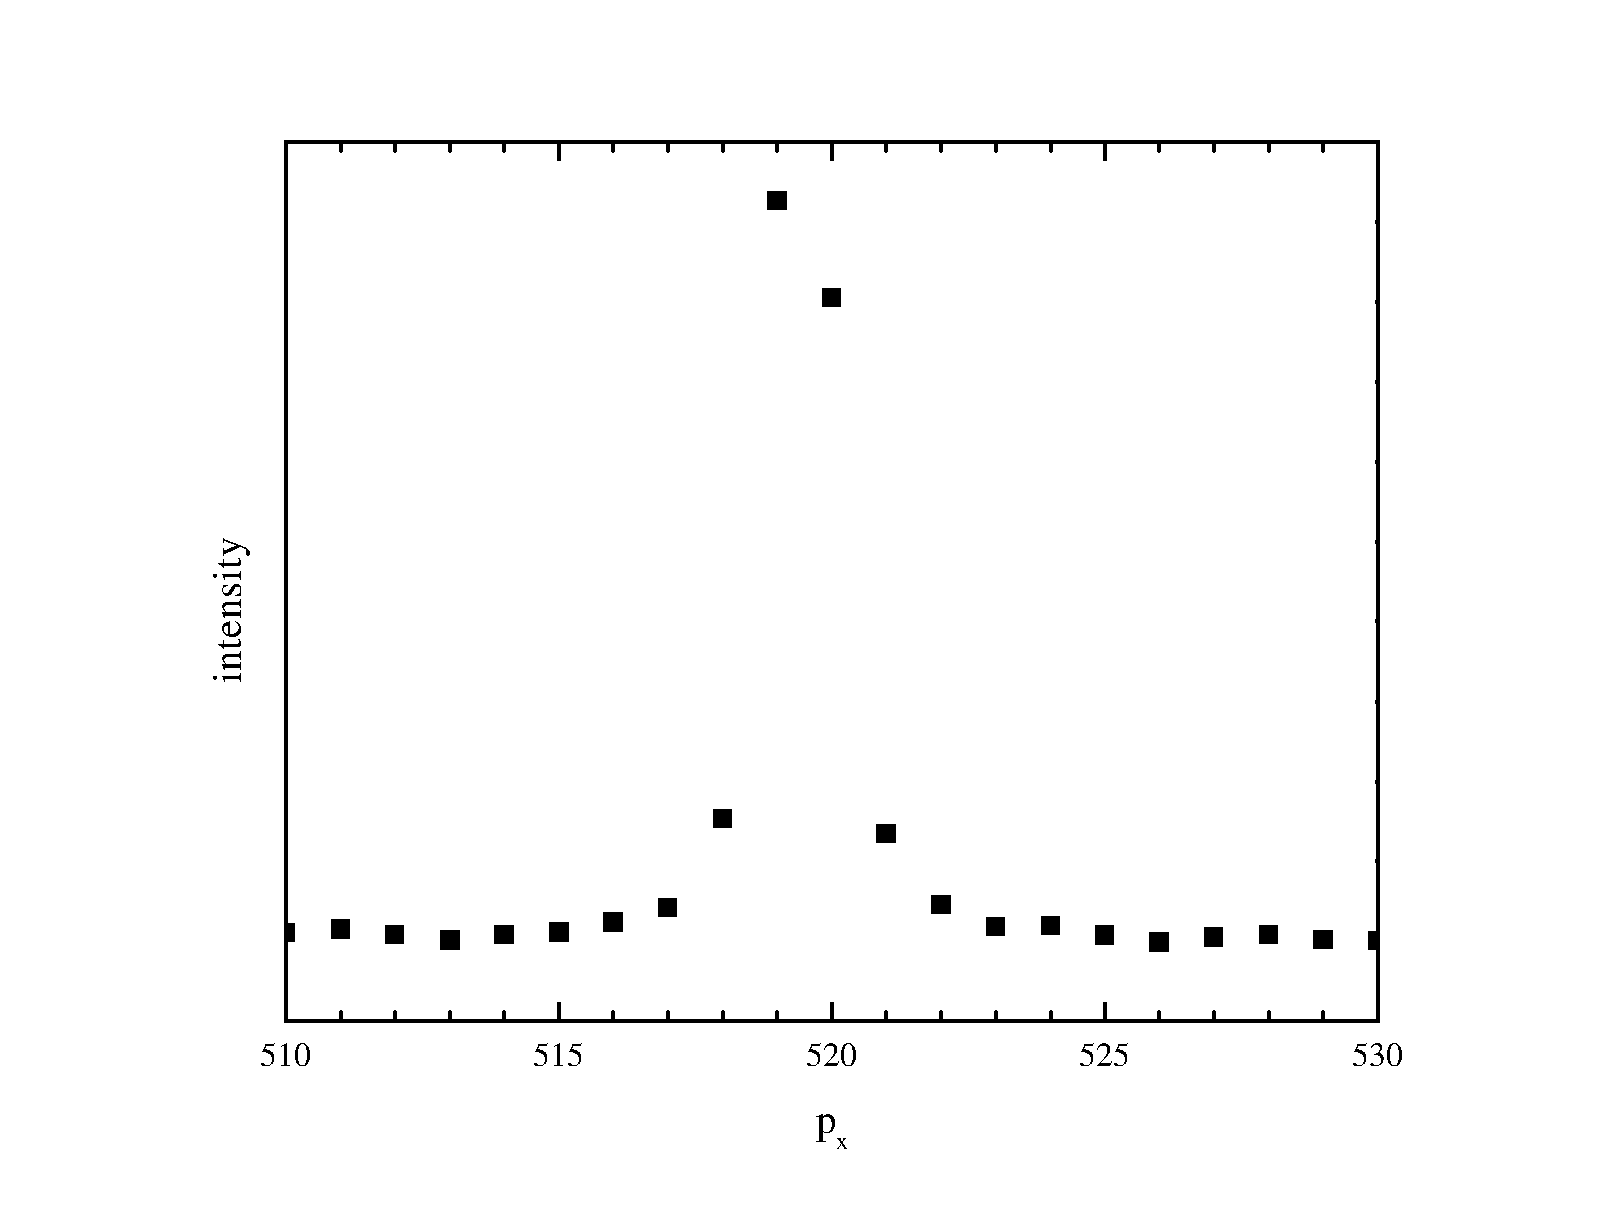
\includegraphics[width=0.45\textwidth]{figures/ripple/beamx_lr}
  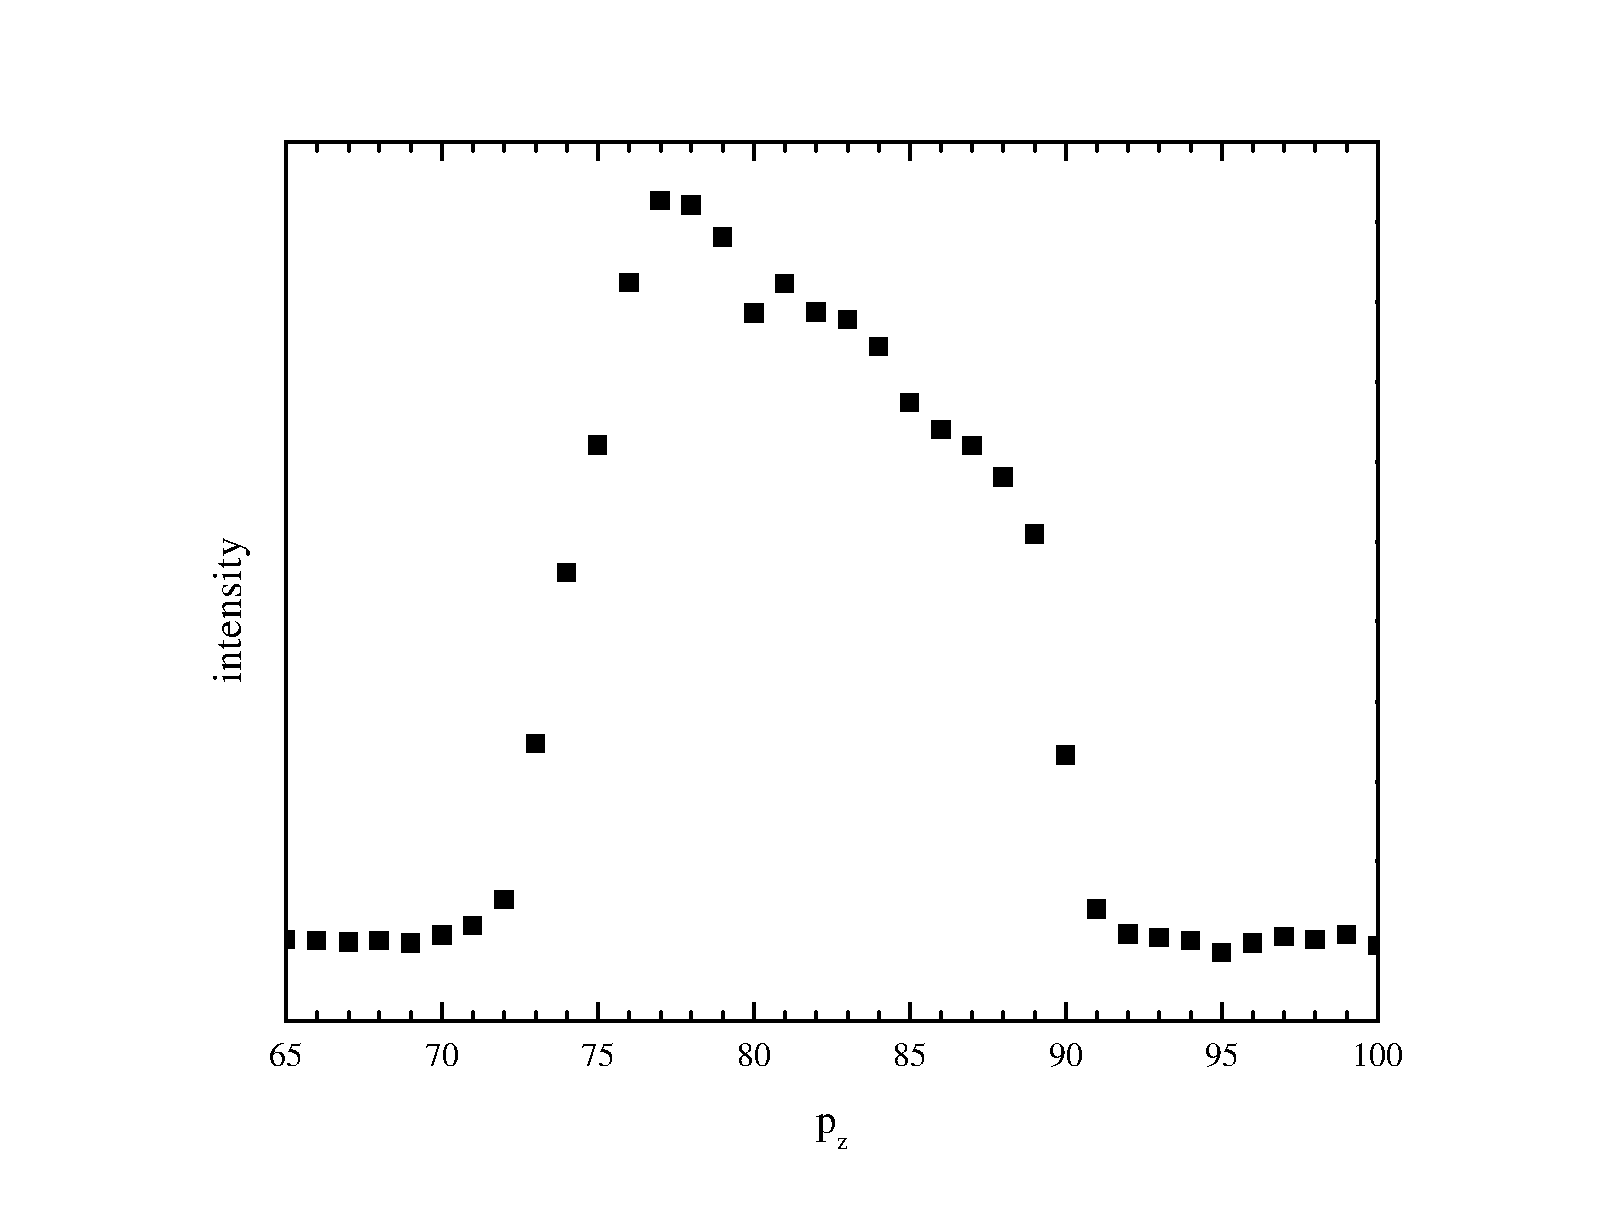
\includegraphics[width=0.45\textwidth]{figures/ripple/beamz_lr}
  \caption{Beam used in the low resolution experiment.
  The horizontal beam profile (left) and vertical beam profile (right)
  are shown.}
  \label{fig:ripple_lr_beam}
\end{figure}

A few Bragg peaks in the low angle X-ray scattering of the ripple phase
were very strong, leading to saturation of CCD pixels for data collection
with a long exposure time. 
In order to probe a wide range of $q$-space, three images were taken:
1) a short, one second exposure with a nominally 25 micron 
molybdinum attenuator installed in the upstream of the sample to reduce the intensity
of the X-ray beam, 2) one second exposure without the beam attenuator,
and 3) 60 second exposure with a beam stop blocking the very intense 
(1,0) and (2,0) peaks. See Fig.~\ref{fig:ripple_laxs_image}. 
Then, the integrated intensity of (1,0) peak was measured
from the first image. This value was multiplied by 6.9 to account for the beam
attenuation and by 60 to scale with the exposure time. 
The intensity of (2,0) and (2,-1) were measured from the second image, also
multiplied by 60 to account for the shorter exposure time. The intensity of
the rest of the observed peaks were measured from the third image.

The integrated intensity of each peak was obtained by putting a box around a
peak and summing up the intensity in those pixels that fall inside the box.
The background scattering was estimated by measuring the intensity in pixels
near the peak but not containing any peak tail. The choice of box size was 
made according to the width of each peak. Because of mosaic spread in the sample,
the peaks were wider for higher orders. 
Consequently, the box was made wider for higher
orders. The box size was chosen so that approximately 80\% of the peak intensity
was counted toward the integrated intensity.

A thin piece of molybdenum was used to attenuate the beam. The attenuation length
$\mu$ of X-ray in Mo is 6.433 $\mu$m for 8 keV and 13.74 $\mu$m for 10.55 keV 
\cite{ref:cxro}.
For a 25 $\mu$m thick Mo attenuator, $\mu=13.74$ gives the attenuation factor 
of $[\exp(-25/13.74)]^{-1} = 6.2$. The exact attenuation factor was determined
by comparing X-ray images collected with and without the attenuator
, shown in Fig.~\ref{fig:attenuator}.
The attenuation factor of the nominally 25 $\mu$m thick Mo was found to 
be 6.9 for the wavelength used (1.175 \AA). 

\begin{figure}
  \centering
  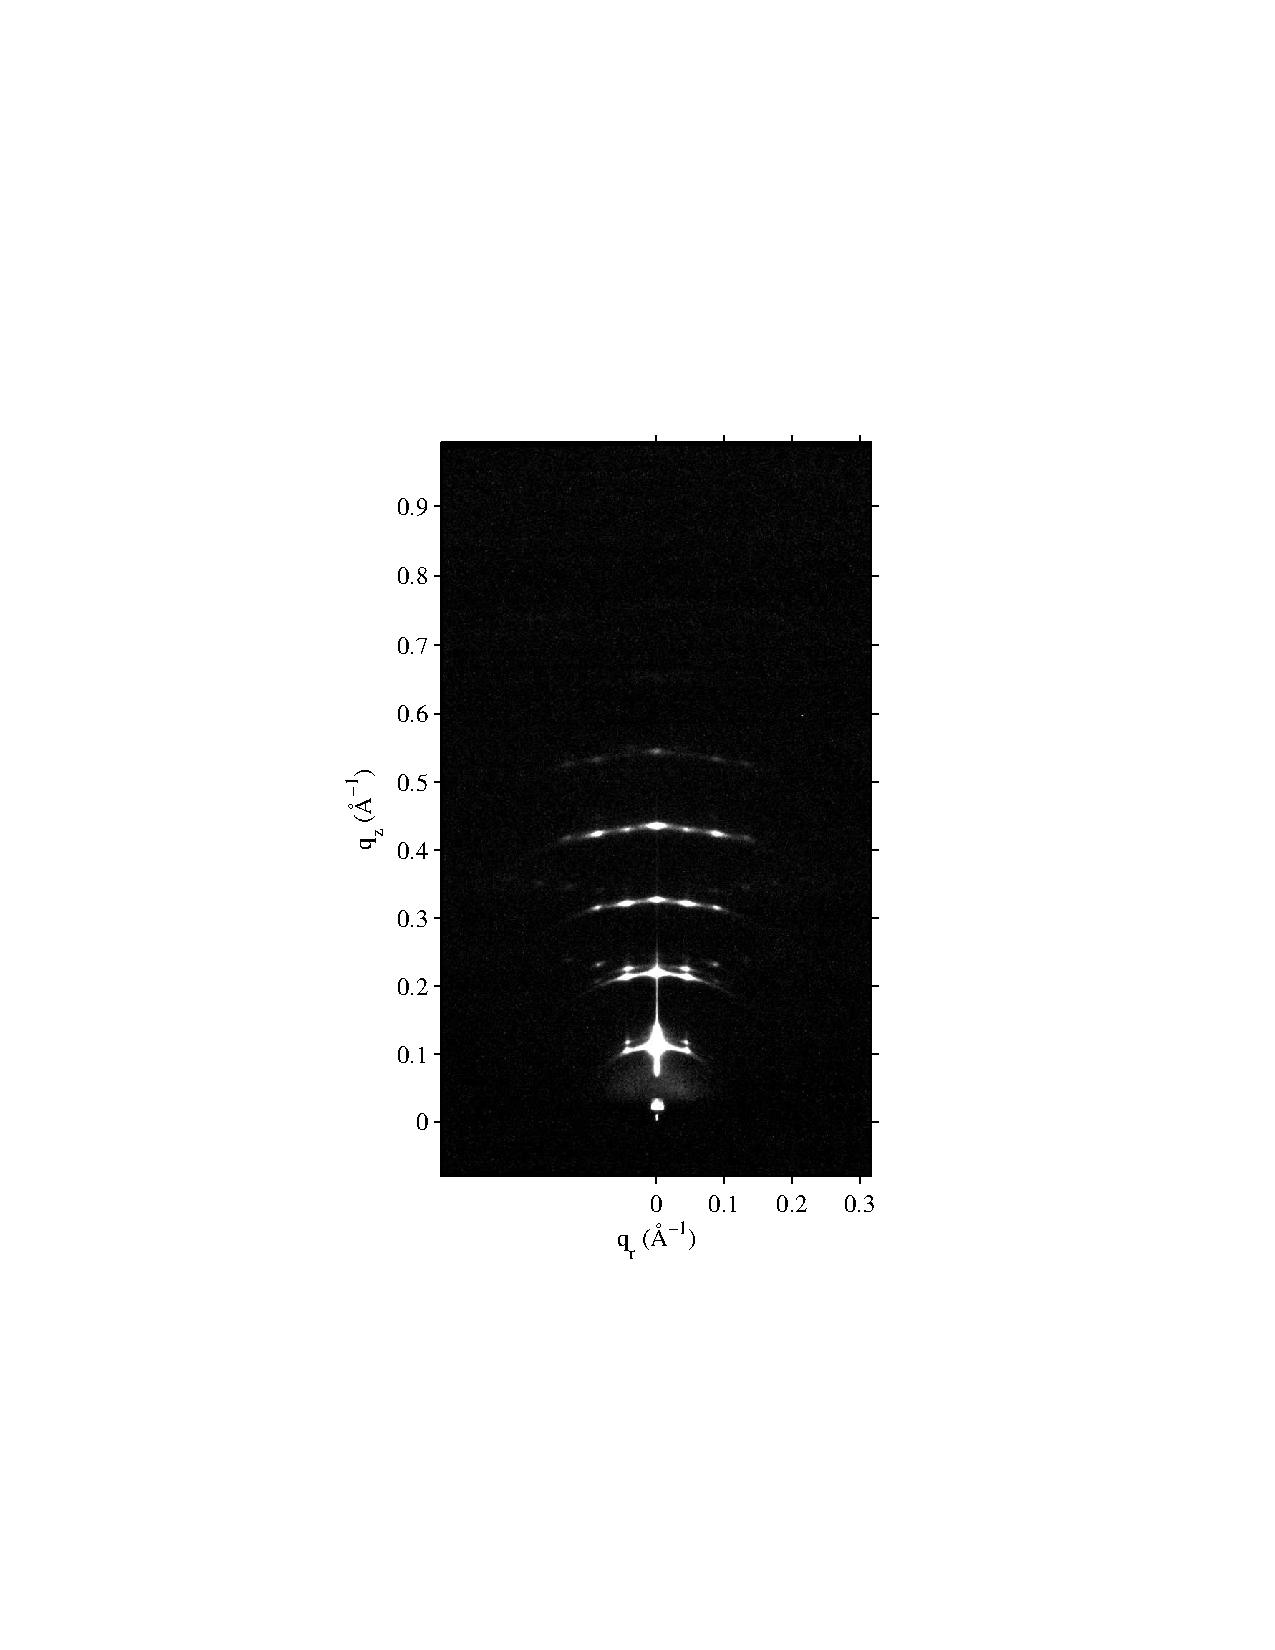
\includegraphics[trim=160 180 160 180,clip,width=0.49\textwidth]{figures/ripple/ripple083}
  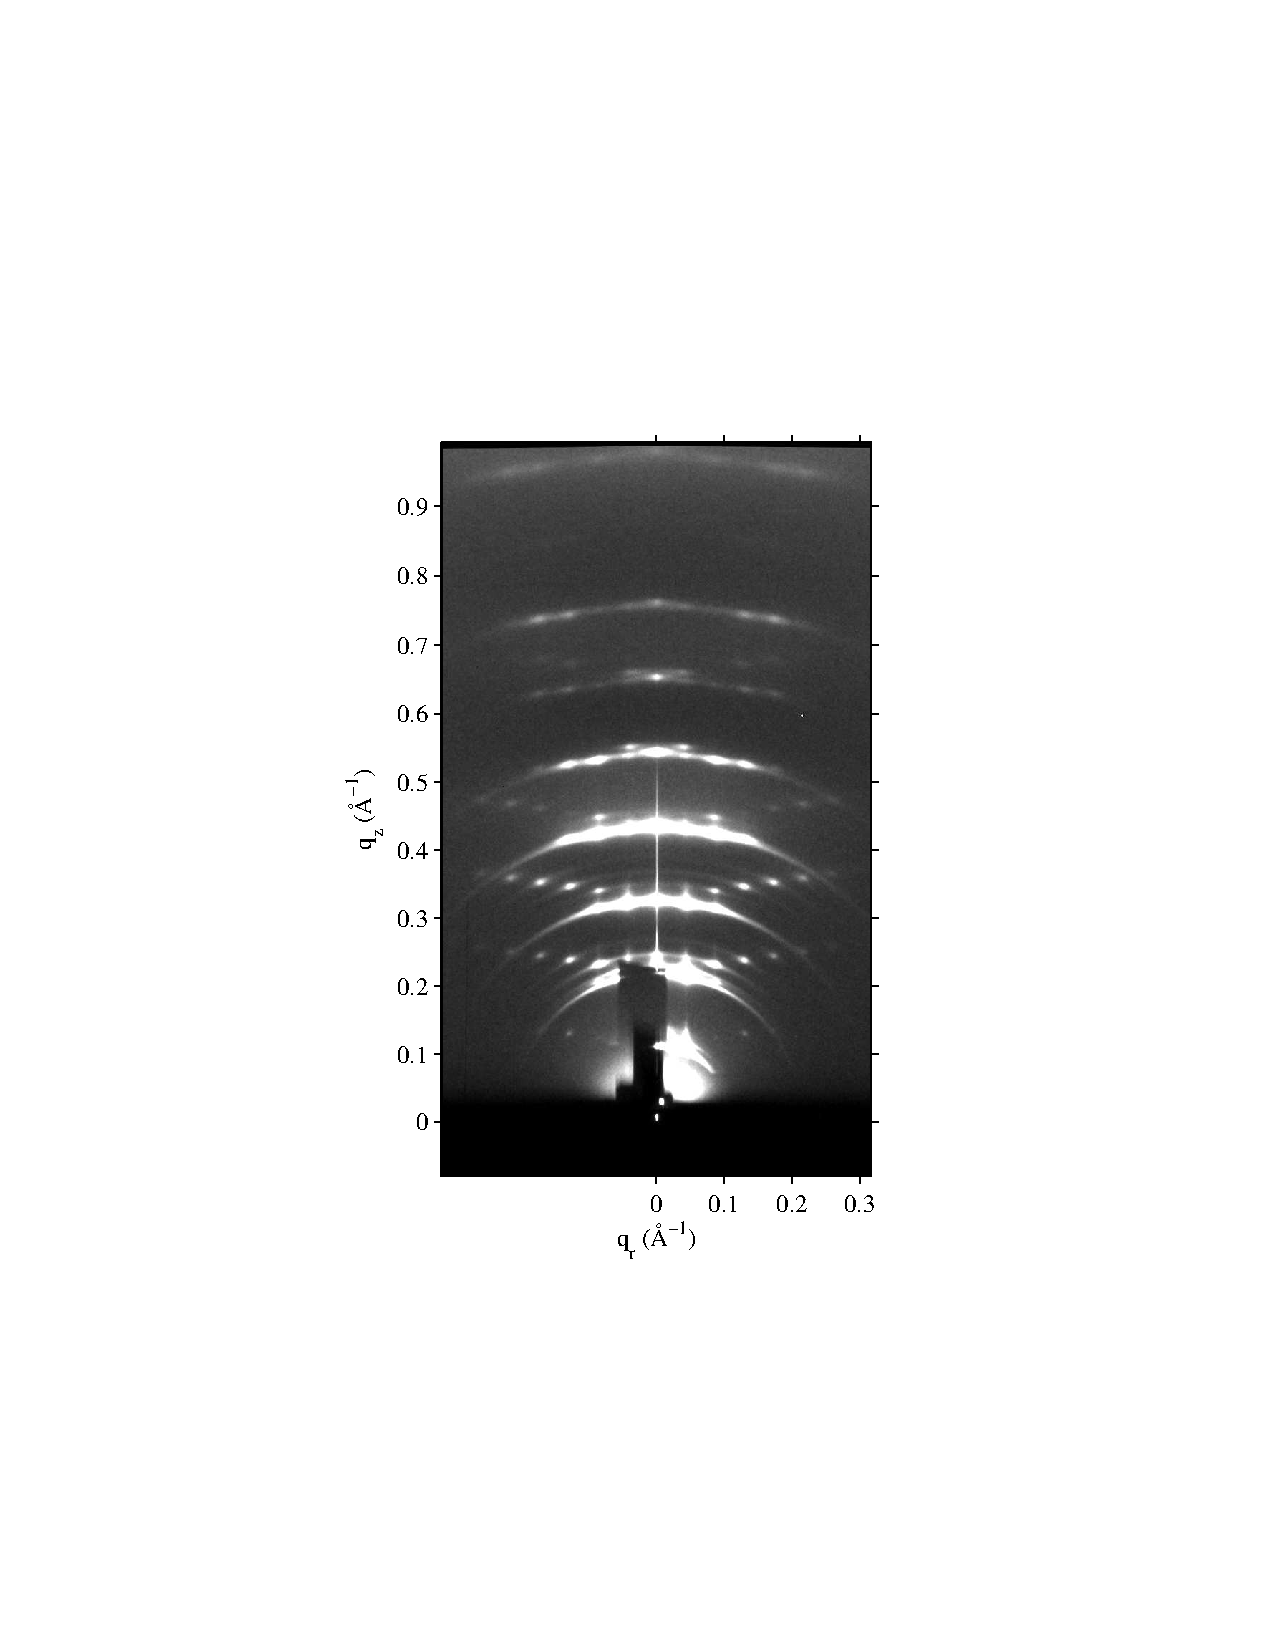
\includegraphics[trim=160 180 160 180,clip,width=0.49\textwidth]{figures/ripple/ripple085}
  \caption{1 second exposure (left) and 60 second exposure (right) of the low
  angle X-ray scattering from the DMPC ripple phase. The dark rectangle 
  in the right image extending from $q_z$ = 0 \AA$^{-1}$ to 0.2 \AA$^{-1}$
  is the shadow cast by 100 $\mu$m thick molybdenum beam stop.
  $D$ = 57.8 \AA, $\lambda_r$ = 145.0 \AA, and $\gamma$ = 97.8\textdegree.
  The gray scales used are [0 100] (left) and [0 500] (right).}
  \label{fig:ripple_laxs_images}  
\end{figure} 

\begin{figure}
  \centering
  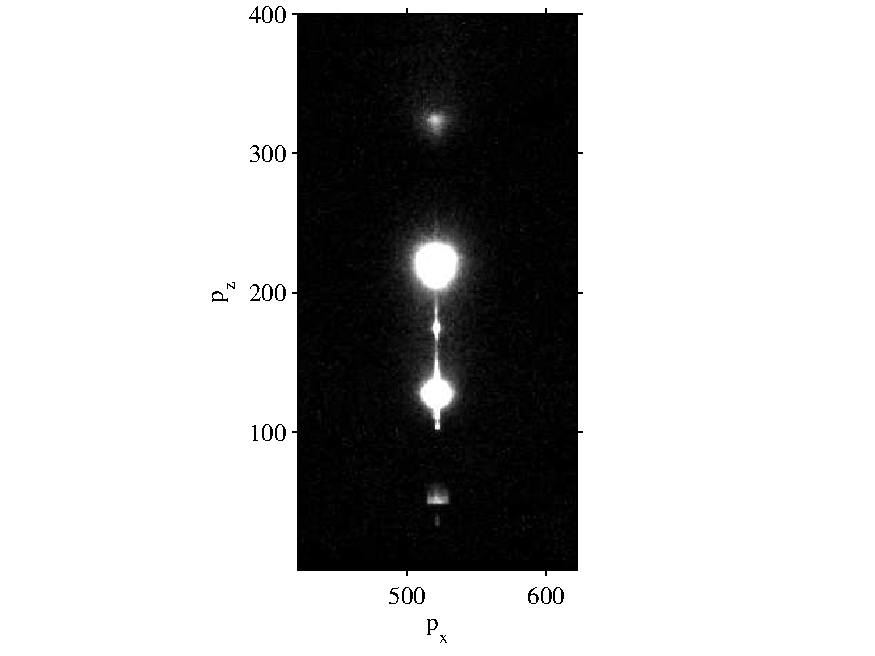
\includegraphics[trim=100 0 100 0,clip,width=0.45\textwidth]{figures/ripple/olddopc045}
  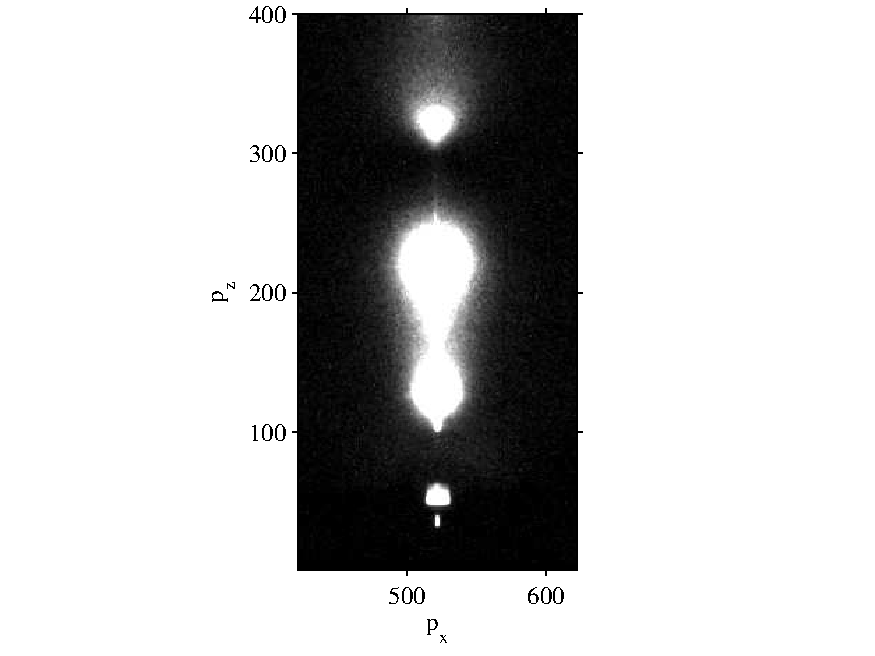
\includegraphics[trim=100 0 100 0,clip,width=0.45\textwidth]{figures/ripple/olddopc044}
  \caption{CCD images of X-ray scattering taken with (left) and without 
  (right) a nominally 25 $\mu$m thick Mo attenuator. These data were taken 
  at a fixed angle of incidence. The sample was an oriented film of 
  DOPC:DOPE (3:1) in the fluid phase at 37 \textcelsius. The wavelength
  was 1.175 \AA, the same as the one used for the ripple phase experiment.
  The same gray scale is used in both images.}
  \label{fig:olddopc}
\end{figure}

\begin{figure}
  \centering
  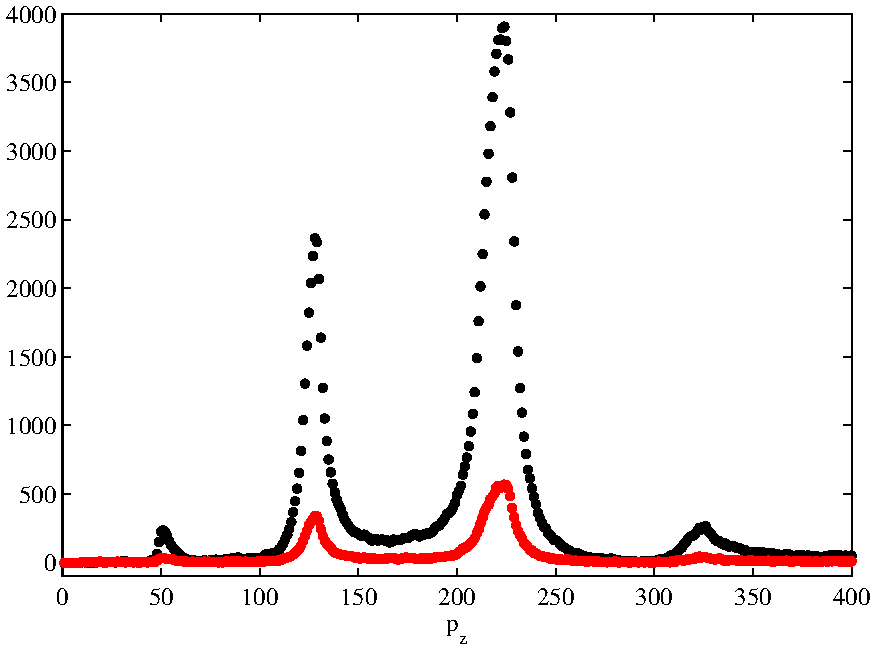
\includegraphics[width=0.45\textwidth]{figures/ripple/attenuator1}
  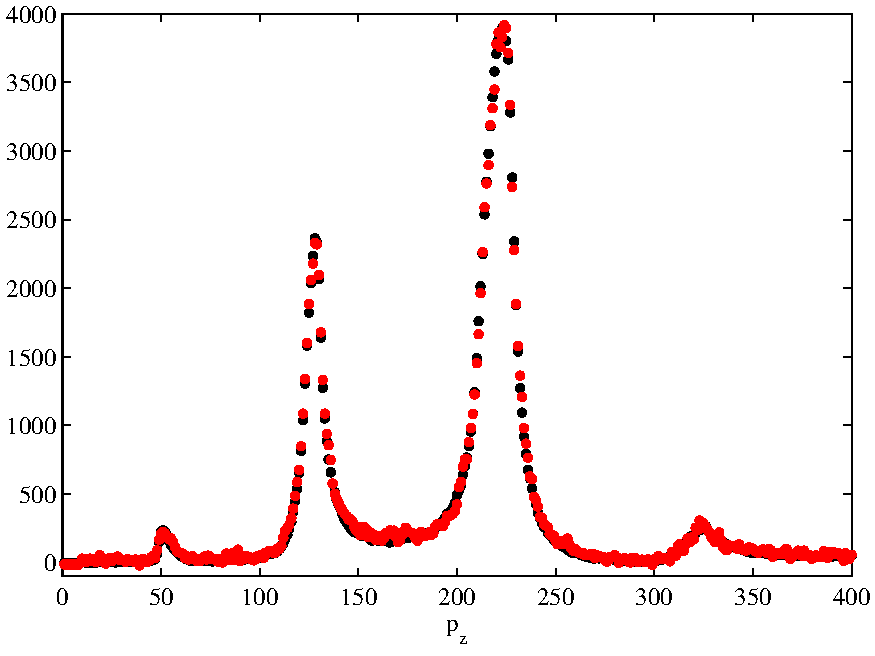
\includegraphics[width=0.45\textwidth]{figures/ripple/attenuator2}
  \caption{Vertical $p_z$ slices of X-ray images shown in Fig.~\ref{fig:olddopc}
  (left). The scattering intensity measured with the attenuator (red solid circles) 
  was multiplied by 
  a factor of 6.9 and compared to the intensity measured 
  without the attenuator (black solid circles, right).}
  \label{fig:attenuator}
\end{figure}

\subsection{Near Grazing Incidence Wide Angle X-ray Scattering Experiment}
The high resolution X-ray scattering experiment was also carried out at 
the G1 station.
The energy of the beam was 10.55 keV (wavelength = 1.175 \AA).
Instead of a multilayer monochromator with 1.5\% energy dispersion, a (111)
silicon monochromator with $\Delta E/E$ of 0.01\% was used to achieve
a higher resolution than that for the low angle X-ray scattering experiment
(section \ref{}).
The horizontal and vertical divergence of the X-ray beam were
$4.2 \times 10^{-5}$ rad and $1.6 \times 10^{-4}$ rad, respectively. 
Because the resolution was dominated by the geometric broadening due to the
sample width along the beam direction, the sample was trimmed to 1 mm.
The width of 1 mm was chosen simply because I could not trim more
without a more sophisticated device than a simple razor blade. Also, a very
narrow sample would be a weak scattering body. Due to limited availability
of synchrotron beam time, I considered 1 mm width to be reasonable.

%S1L = 153.6 mm, S1H = 220.6 mm, and S2 = 359.7 mm
The sample to detector distance was 220.6 mm, measured using a silver behenate film. 
The horizontal beam width was 0.2 mm. Wide angle X-ray
scattering was collected at an incident angle of 0.2\textdegree. 

\begin{figure}
  \centering
  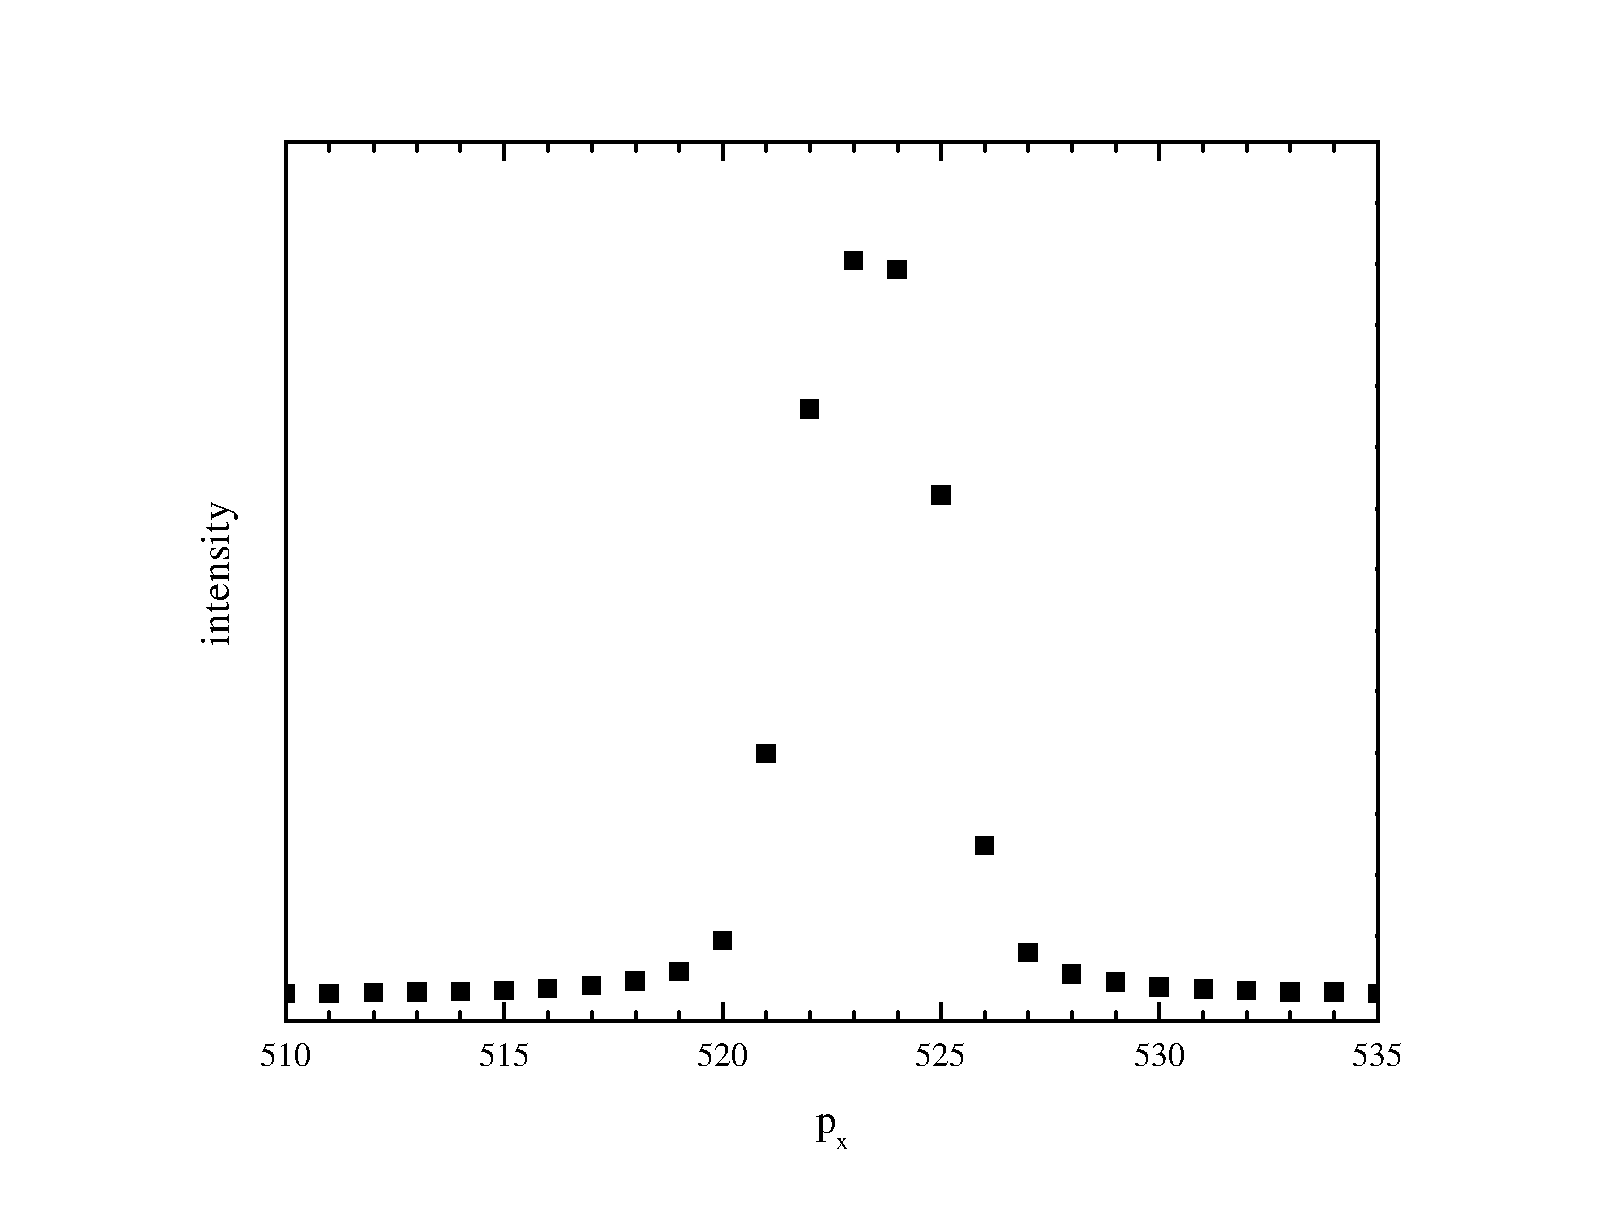
\includegraphics[width=0.45\textwidth]{figures/ripple/beamx_hr}
  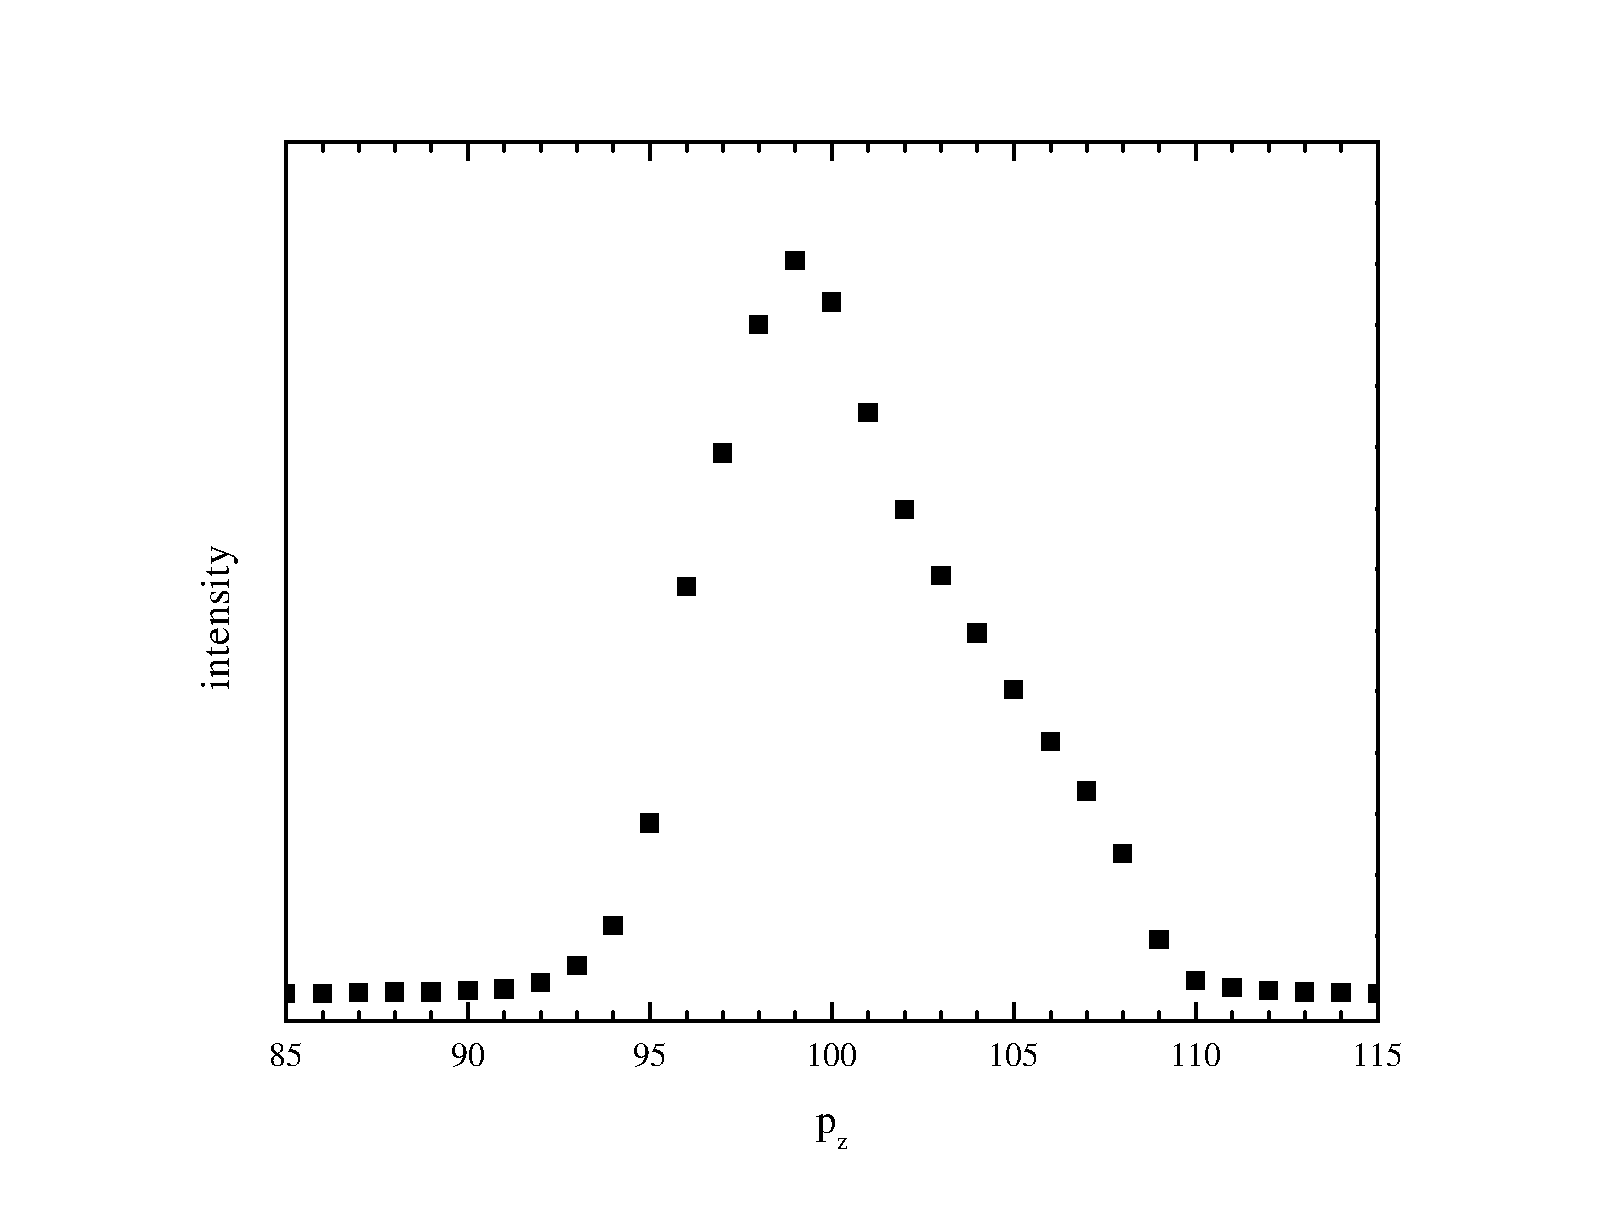
\includegraphics[width=0.45\textwidth]{figures/ripple/beamz_hr}
  \caption{Beam used in the high resolution experiment.
  The horizontal beam profile (left) and vertical beam profile (right)
  are shown.}
  \label{fig:NGIWAXS_beam}
\end{figure}

\subsection{Transmission Wide Angle X-ray Scattering Experiment}
The energy of the beam was 10.5 keV. A W/B$_4$C multilayer monochromator
with an energy dispersion of 1.5\% was used. The sample to detector
distance was measured to be 170 mm using a sliver behenate 
when the angle of incidence $\omega$ was 0\textdegree.
The incident angle was set to -45\textdegree\ for transmission data
collection. A 35 $\mu$m thick silicon substrate absorbs an X-ray at
10.5 keV by 20\%\ \cite{ref:cxro}. 
To measure a D-spacing, mosaic spread of the sample was exploited. Because 
the axis of the rotation motor did not coincide with the sample axis,
the sample to detector distance varied as $\omega$ was varied. To accurately
measure the sample to detector distance, low angle scattering was collected
at a fixed $\omega$. Due to the sample mosaic spread, many orders were
visible. While the relative intensity of each order was inaccurate, 
the position of peaks was the same as that observed with a rotating sample.
The sample to detector distance was accurately measured at $\omega$ = 0\textdegree
usign a silver behenate sample. From the geometry of the sample holder,
a shift in the sample to detector distance was estimated for an arbitrary 
incident angle $\omega$.

Explain how we estimated the sample to detector distance at
$\omega$ = -45\textdegree. Explain how we leveled the sample 
(using the sample scattering and ascan).
The background scattering was collected by replacing the sample with a bare 
wafer.

\begin{figure}
  \centering
  \caption{The sample holder geometry. Copy a figure from my old writeup.}
  \label{fig:sample_holder}
\end{figure}

%%%%%%%%%%%%%%%%%%%%%%%%%%%%%%%%%%%%%%%%%%%%%%%%%%%%%%%%%%%%%%%%%%%%%%%%%%%%%%%
\section{Some Theories}\label{sec:some_theories}
\subsection{Lattice Structure}\label{sec:lattice_structure}
It has been shown from X-ray studies (ref) that ripples in in different bilayers
are registered to form a two-dimensional oblique lattice as shown by the unit 
cell in Fig. X. 
The unit cell vectors in the ripple phase can be expressed as 
\begin{equation}
  \mathbf{a} = \frac{D}{\tan\gamma}\xhat + D\zhat
\end{equation}
and
\begin{equation}
  \mathbf{b} = \lambda_r\xhat.
\end{equation}
The corresponding reciprocal lattice unit cell vectors are
\begin{equation}
  \mathbf{A} = \frac{2\pi}{D}\zhat
\end{equation}
and
\begin{equation}
  \mathbf{B} = \frac{2\pi}{\lambda_r}\xhat - \frac{2\pi}{\lambda_r\tan\gamma}\zhat.
\end{equation}
The reciprocal lattice vector, $\mathbf{q}_{hk}$ for the Bragg peak with 
Miller indices $(h,k)$ is 
\begin{equation}
  \mathbf{q}_{hk}=h\mathbf{A}+k\mathbf{B},
\end{equation}
so its Cartesian components are
\begin{align}
  & \mathbf{q}_{hk}\cdot\xhat = q_{hk}^x = \frac{2\pi k}{\lambda_r} \equiv q_{k}^x \\
  & \mathbf{q}_{hk}\cdot\yhat = q_{hk}^y = 0 \\
  & \mathbf{q}_{hk}\cdot\zhat = \qz{hk} = \frac{2\pi h}{D} - \frac{2\pi k}{\lambda_r\tan\gamma}.
\end{align}

%%%%%%%%%%%%%%%%%%%%%%%%%%%%%%%%%%%%%%%%%%%%%%%%%%%%%%%%%%%%%%%%%%%%%%%%%%%%%%%
\subsection{Sample $q$-space}
The incoming and outgoing wavevectors of the x-ray beam in Fig. XXX 
are given by
\begin{equation}
  \kin = \frac{2\pi}{\lambda} \yhat, \quad
  \kout = 
    \frac{2\pi}{\lambda} \left( 
      \sin 2\theta \cos\phi \, \xhat
      + \cos 2\theta \, \yhat
      + \sin 2\theta \sin\phi \, \zhat 
    \right),
  %\label{eq:kinkout}
\end{equation}
where $\lambda$ is the wavelength of x-ray, $2\theta$ is the total scattering
angle, and $\phi$ is the angle measured from the equator on the detector. 
The scattering vector (also called
momentum transfer vector) is
the difference between $\kin$ and $\kout$,
\begin{align}
  \mathbf{q} &= \kout - \kin \nonumber \\
             &= q \left( 
                  \cos\theta\cos\phi \, \xhat - \sin\theta \, \yhat
                  + \cos\theta\sin\phi \, \zhat
                \right),
  \label{eq:q_vector}
\end{align}
where $q=4\pi\sin\theta/\lambda$ is the magnitude of the scattering vector. 
When the sample is rotated by $\omega$ about the lab x-axis in the clockwise 
direction as shown in Fig. XXX, the sample $q$-space also rotates and 
are given by  
\begin{equation}
  \mathbf{\hat{e}_x} = \xhat, \quad
  \mathbf{\hat{e}_y} = \cos\omega\,\yhat + \sin\omega\,\zhat, \quad
  \mathbf{\hat{e}_z} = -\sin\omega\,\yhat + \cos\omega\,\zhat.
  \label{eq:smp_coord}
\end{equation}
From Eq.~(\ref{eq:q_vector}) and (\ref{eq:smp_coord}), we find the sample
$q$-space to be
\begin{align}
  q_x &= \mathbf{q}\cdot\mathbf{\hat{e}_x} 
       = q\cos\theta\cos\phi, 
       \nonumber\\
  q_y &= \mathbf{q}\cdot\mathbf{\hat{e}_y} 
       = q\left(-\sin\theta\cos\omega + \cos\theta\sin\phi\sin\omega\right), 
       \nonumber\\
  q_z &= \mathbf{q}\cdot\mathbf{\hat{e}_z} 
       = q\left(\sin\theta\sin\omega + \cos\theta\sin\phi\cos\omega\right).
       \label{eq:qxqyqz}
\end{align}
The position, $(X,Z)$, of a CCD pixel is measured with respect to the beam 
and given by
\begin{equation}
  X = S \tan 2\theta \cos\phi, \quad Z = S \tan 2\theta \sin\phi,
  \label{eq:XZ}
\end{equation} 
where $S$ is the distance between the sample and detector.
From a model for the electron density of a lipid bilayer, one calculates
a X-ray scattering intensity pattern, $I(\mathbf{q})$. Then, Eq.~(\ref{eq:qxqyqz})
and (\ref{eq:XZ}) relate $I(\mathbf{q})$ to the experimentally measured
intensity pattern, $I(X,Z)$. It is important to remember that a given pixel
position, $(X,Z)$, corresponds to a triplet $(q_x, q_y, q_z)$. Fully exploring 
the sample $q$-space requires changing $\omega$ for a fixed wavelength, which was
achieved by continuously rotating the sample with a motor. In the ripple phase, 
because our sample has in-plane rotational symmetry,
the ripple side peaks make up Bragg rings while the main peaks are still 
delta function like (see Fig. X) in $q$-space. In order for the main peak to be
observed, $\omega$ must be equal to $\theta_\mathrm{B}$, but the side peaks
are observed at any $\omega$. Those side peaks get slightly smeared due to 
integration over $q_y$.

For low angle x-ray scattering (LAXS), it is convenient to linearize the above
equations in terms of $\theta$ and $\omega$. In the small angle approximation, 
$\sin\phi \approx Z/(2S\theta)$ and $\cos\phi \approx X/(2S\theta)$, and
\begin{align}
  q_x &\approx \frac{4\pi\theta\cos\phi}{\lambda} \approx kX/S \nonumber\\
  q_y &\approx q_z\omega -\frac{4\pi\theta^2}{\lambda} \approx q_z\omega - \frac{\lambda q_z^2}{4\pi}\nonumber\\
  q_z &\approx \frac{4\pi\theta\sin\phi}{\lambda} \approx kZ/S,
  \label{eq:qxqyqz_small}
\end{align}
with $k=2\pi/\lambda$. For wide angle X-ray scattering, the exact relations given
by Eq.~(\ref{eq:qxqyqz}) are necessary. Especially in the transmission experiment,
where $\omega$ is large, an observed X-ray pattern appears nontrivial and becomes
almost impossible to analyze without the use of Eq.~(\ref{eq:qxqyqz}).


%%%%%%%%%%%%%%%%%%%%%%%%%%%%%%%%%%%%%%%%%%%%%%%%%%%%%%%%%%%%%%%%%%%%%%%%%%%%%%%
\subsection{Lorentz Correction}\label{sec:Lorentz_correction}
Our sample has in-plane rotational symmetry. This means that the sample 
consists of many domains with differing ripple directions, all domains
being parallel to the substrate.  
In sample $q$-space, then, ripple side peaks become rings while main peaks are
still points (see Fig. X). For an arbitrary incident angle, main peaks are not observed
while side peaks are observed. 
In order to capture both main and side peaks in one X-ray exposure, 
the sample was continuously rotated. As a result of this rotation, 
main peaks become arcs that subtend an angle $2\theta_{h0}$,
as shown in Fig.~\ref{fig:ewald_main}, with its length
equal to $2\theta_{h0}\qz{h0}$.  

The detector records the cross sections of these arcs with the 
Ewald sphere, so the total scattering power is the product of the observed intensity,
$\Io{hk}$ with the arc length, that is, 
\begin{equation}
  I = 2\theta_{h0}\qz{h0} \Io{h0}. \label{eq:main_ewald}
\end{equation}

Because the sample has in-plane rotational symmetry, side peaks are represented as
rings whose radius is $\qr{hk}$. For a fixed incident
angle, all the rings are intersected by the Ewald sphere. Because only the domains
with the right ripple direction can satisfy the Bragg's condition at a given fixed
angle, the scattering power of this small cross section is reduced by 
a factor of $2\pi \qr{k}$ compared to main peaks. During 
an X-ray exposure, the rings cross the Ewald sphere
at all incident angles. Then, the total scattering power is given by
\begin{equation}
  I=2\pi \qr{k} \Io{k}. \label{eq:side_ewald}
\end{equation}
Inverting Eq.~(\ref{eq:main_ewald}) and (\ref{eq:side_ewald}) 
and realizing that the intensity is the form factor
squared, we can calculate the observed intensity, $\Io{}$, 
from a model for an electron density in the ripple phase.

%------------------------------------------------------------------------------
\begin{figure}[htbp]
  \centering
  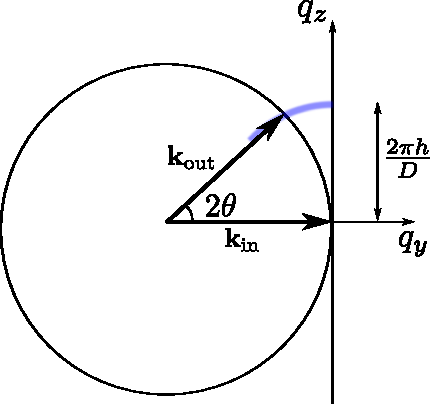
\includegraphics[scale=1]{figures/ripple/ewald_main}
  \caption{caption goes here}
  \label{fig:ewald_main}
\end{figure}
%------------------------------------------------------------------------------

%------------------------------------------------------------------------------
\begin{figure}[htbp]
  \centering
  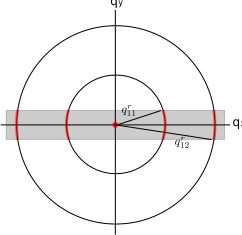
\includegraphics[scale=1]{figures/ripple/ewald_side_h1_ver1}
  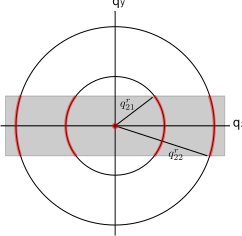
\includegraphics[scale=1]{figures/ripple/ewald_side_h2_ver1}
  \caption{$q$-space representations of Bragg peaks and Bragg rings 
  for $h=1$ and $k$ = 0, 1, and 2 in $\qz{hk}$ planes.
  The shaded rectangles show cross sections of the rotating Ewald sphere along
  $\qz{hk}$ plane. The intersection between the Ewald sphere and 
  a Bragg peak/ring is indicated in red. 
  The observed intensity for the $k\neq 0$ orders is proportional to
  the fraction of the length of red arcs in the circumference. This 
  fraction is equal to one for a $k=0$ order.
  Because the orders are not in the same $q_z$ plane, the range of $q_y$ 
  integration indicated by the height of the rectangle is different for different
  orders. The magnitude of curvature of arcs is exaggerated.}
  \label{fig:ewald_side_h1}
\end{figure}
%------------------------------------------------------------------------------

Mathematically, the rotation is  
equivalent to an integration over $\omega$. In low angle X-ray scattering, 
$q_z$ is constant at a given pixel as $\omega$ is changed, which can be seen from 
Eq.~(\ref{eq:qxqyqz_small}). $\omega$ dependence appears only through $q_y$, 
so rotating the sample is realized by integrating over $q_y$. 
To derive the integration limits, let us consider two cases: (a) When $\omega \leq 0$,
the incoming X-ray beam is blocked by the back of the substrate. This sets 
the lower limit to 0. (b) When $\omega \geq 2\theta$, the substrate blocks 
the outgoing X-ray. Within the small angle approximation, then, $\omega_{\text{max}}$
is $2\times \lambda q_z/(4\pi)$ for scattering with $q_z$. 
Thus, the integration limits 
for $q_y$ integration are $[-\lambda q_z^2/(4\pi), \lambda q_z^2/(4\pi)]$.
We also need to integrate over $X$ and $Z$ to obtain integrated intensity. 
These lead to the observed intensity
written as,
\begin{align}
  \Io{hk} 
    &\propto \int dX \int dZ \int d\omega |F_{hk}|^2 S_{hk}(\mathbf{q}) \nonumber \\
    &\propto |F_{hk}|^2 \int dq_x \int dq_z 
             \int_{-\frac{\lambda q_z^2}{4\pi}}^{\frac{\lambda q_z^2}{4\pi}} 
             \frac{dq_y}{q_z} 
             S_{hk}(\mathbf{q}),
\end{align}
where $1/q_z$ factor in $q_y$ integration is the Lorentz polarization factor
in the small angle approximation. 

For a crystalline sample with the in-plane rotational symmetry, the
structure factor is  
\begin{equation}
  S_{hk}(\mathbf{q}) = S_{hk}(q_r,q_z) 
  = \frac{1}{2\pi q_r}\delta(q_r-q_{r,k})\delta(q_z-q_{z,hk}),
\end{equation} 
where $q_{r,k}=2\pi |k|/\lambda_r$. Thus, the scattering pattern in the 
ripple phase is a 
collection of Bragg ``rings'' centered at the meridian and the 
Bragg peaks located along the meridian.  
The observed, integrated intensity of $hk$ peak is proportional to
\begin{equation}
  I_{\mathrm{o},hk} 
    \propto \frac{\lvert F_{hk} \rvert^2}{q_{z,hk}} \int\mathop{dq_x} 
            \int_{-q_{y0}}^{q_{y0}}
            \mathop{dq_y} \frac{\delta(q_r-q_{r,k})}{2\pi q_r},
\end{equation}
where $q_{y0} = \lambda q_{z,hk}^2/(4\pi)$.
For side peaks ($k \neq 0$), we have 
\begin{align}
  \int\mathop{dq_x} \int_{-q_{y0}}^{q_{y0}}\mathop{dq_y} \frac{\delta(q_r-q_{r,k})}{2\pi q_r}
  &\approx \int_{-\frac{q_{y0}}{q_{r,k}}}^{\frac{q_{y0}}{q_{r,k}}} \mathop{d\phi} 
          \int \mathop{dq_r} q_r\frac{\delta(q_r-q_{r,k})}{2\pi q_r} \nonumber\\
 &= \frac{q_{y0}}{\pi q_{r,k}}. \label{eq:side_integrand}
\end{align}
For main peaks ($k=0$), we have 
\begin{align}
  \int\mathop{dq_x} \int_{-q_{y0}}^{q_{y0}}\mathop{dq_y} \frac{\delta(q_r-q_{r,k})}{2\pi q_r}
  &= \int_0^{2\pi}\mathop{d\phi} \int\mathop{dq_r} q_r\frac{\delta(q_r-q_{r,k})}{2\pi q_r} \nonumber\\
  &= 1 \label{eq:main_integrand}
\end{align}
Using Eq.~(\ref{eq:side_integrand}) and (\ref{eq:main_integrand}), 
we write the observed integrated intensity as
\begin{align}
  I_{\mathrm{o},h0} &\propto \frac{|F_{h0}|^2}{q_{z,h0}} \label{eq:main}\\
  I_{\mathrm{o},hk} &\propto \frac{|F_{hk}|^2}{q_{z,hk}} \frac{q_{y0}}{\pi q_{r,k}}
    = |F_{hk}|^2 \frac{\lambda q_{z,hk}}{2\pi}\frac{1}{2\pi q_{r,k}}
    = |F_{hk}|^2 \frac{2\theta_{hk}}{2\pi q_{r,k}}, \label{eq:side}
\end{align}
where $2\theta_{hk} = \lambda q_{z,hk}/(2\pi)$ is the incident angle at which 
the outgoing X-ray for the peak $(hk)$ is blocked by the substrate.
Eq.~(\ref{eq:main}) and (\ref{eq:side}) relate the form factor calculated from
a model to the experimentally observed intensity, and are 
equivalent to Eq.~(\ref{eq:main_ewald}) and (\ref{eq:side_ewald}), 
which were derived by using the Ewald sphere. 

In non-linear least squares fitting procedure, 
we fitted the observed integrated intensity to
the calculated intensity from a bilayer model using these geometrical corrections. 
This is because we can determine experimental uncertainties
on observed intensity rather than the geometrically corrected form factors. 
We avoid propagating the uncertainties by fitting a model to observed intensity. 

%%%%%%%%%%%%%%%%%%%%%%%%%%%%%%%%%%%%%%%%%%%%%%%%%%%%%%%%%%%%%%%%%%%%%%%%%%%%%%%
\subsection{Absorption Correction for LAXS}
In this section, we derive the absorption correction for the thin film
sample. The calculation involves an explicit integration over the incident angle, 
$\omega$, which is necessiated by the sample rotation during an x-ray exposure. 
The procedure is to write down an absorption factor, $A(\omega,\theta)$, for a 
given scattering angle at a given incident angle, and
then integrate over $\omega$. We ignore $q_x$ dependence because the X-ray
path inside the sample is nearly within the $y$-$z$ plane for low angle
scattering. The correction for wide angle scattering is described in a later
section.

Assume that all the X-rays enter the sample from the top surface. The total scattering
angle is given by $2\theta$ (see Fig.~\ref{fig:absorption_LAXS}).
%------------------------------------------------------------------------------
\begin{figure}[htbp]
  \centering
  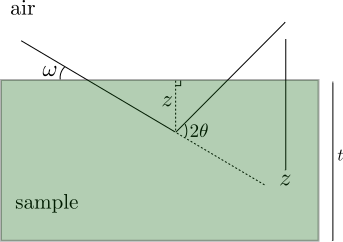
\includegraphics[scale=1]{figures/ripple/absorption_LAXS}
  \caption{The path of X-rays within the sample. The incident angle is 
  $\omega$ and the total scattering angle is $2\theta$. An X-ray with a
  penetration depth of $z$ is shown. The total thickness of the sample
  is $t$.}
  \label{fig:absorption_LAXS}
\end{figure}
%------------------------------------------------------------------------------
Let $z$-axis point downward. At the top surface
(air-sample interface), $z=0$. For X-rays that travel to $z$ and then scatter, the
total path length within the sample is 
\begin{equation}
  L_\textrm{tot}(z,\omega,\theta) 
  = \frac{z}{\sin\omega}+\frac{z}{\sin(2\theta-\omega)} 
  = zg(\omega,\theta),
\end{equation}
where $g(\omega,\theta)=(\sin\omega)^{-1}+\pars{\sin\pars{2\theta-\omega}}^{-1}$.
For each ray, the intensity is attenuated by the sample absorption. 
If non-attenuated 
intensity is equal to $I_0$, then the attenuated intensity is
\begin{equation}
  I(z,\omega,\theta) = I_0\exp\left(-\frac{L_\textrm{tot}}{\mu}\right),
  \label{eq:ray}
\end{equation}
where $\mu$ is the absorption length of an X-ray. $\mu$ is 111 for 10.5 keV
and 222 for 8 keV \cite{ref:cxro}.
The observed intensity of scattering from a sample fixed at an angle $\omega$ 
is equal to the integration
of Eq.~(\ref{eq:ray}) over the whole sample and given by
\begin{align}
  I_{\textrm{obs}}(\omega,\theta) 
    &= \int_0^t \dz I(z,\omega,\theta)
     = I_0\int_0^t\dz \exp\left(-\frac{g(\omega,\theta)}{\mu}z\right) \nonumber \\
    &= I_0\mu \frac{1-\exp\left(-\frac{t}{\mu}g(\omega,\theta)\right)}{g(\omega,\theta)}.
    \label{eq:I_obs1}
\end{align}
Defining the absorption factor at a fixed angle to be $A(\omega,\theta)$, 
the observed intensity can be written as
\begin{equation}
I_{\textrm{obs}}(\omega,\theta)=A(\omega,\theta)tI_0,
\label{eq:I_obs2}
\end{equation}
where $tI_0$ is the intensity we would observe for non-absorbed X-rays.
Equating Eq.~(\ref{eq:I_obs1}) and (\ref{eq:I_obs2}), we get
\begin{equation}
  A(\omega,\theta) = \frac{\mu}{t} 
                     \frac{1-\exp\left(-\frac{t}{\mu}g(\omega,\theta)\right)}{g(\omega,\theta)}.
\end{equation}
The total observed intensity from a sample that is being rotated during 
an exposure is simply
\begin{equation}
  I_{\textrm{total}}(\theta) 
  = \int_0^{2\theta}\textrm{d}\omega I_{\textrm{obs}}(\omega,\theta).
\end{equation}
The upper integration limit is equal to $2\theta$ because the substrate
completely blocks the scattered X-rays above this angle as discussed in 
section \ref{sec:Lorentz_correction}.

Because the total non-attenuated intensity is given by $t\omega I_0$,


so that the total absorption factor is equal to
\begin{equation}
  A(\theta) = \frac{\mu}{2\theta t} \int_0^{2\theta}d\omega 
      \frac{1-\exp\left(-\frac{t}{\mu}g(\omega)\right)}{g(\omega)}.
\end{equation}
If $\mu$ is taken to infinity (no absorption), $A$ goes to 1 as expected. 
Here, it is important to note that $1/2\theta$ factor in the above equation
is normally called Lorentz polarization factor, which
is usually approximated as $1/q_z$ for LAXS analysis. Since the SDP
program applies this correction factor in addition to the absorption
correction, we remove this factor in the formula for $A_c$. Therefore,
the final result for the total absorption correction is 
\begin{equation}
  A_c(\theta) 
    = \frac{1}{2\theta A(\theta)} \nonumber \\
    = \frac{t}{\mu} 
       \left[ 
         \int_0^{2\theta}d\omega 
         \frac{1-\exp\left(-\frac{t}{\mu}g(\omega)\right)}{g(\omega)}
       \right]^{-1}
\end{equation}
with $g(\omega)=1/\sin\omega+1/\sin(2\theta-\omega)$.

%%%%%%%%%%%%%%%%%%%%%%%%%%%%%%%%%%%%%%%%%%%%%%%%%%%%%%%%%%%%%%%%%%%%%%%%%%%%%%%
\subsection{Absorption Correction for WAXS}

%%%%%%%%%%%%%%%%%%%%%%%%%%%%%%%%%%%%%%%%%%%%%%%%%%%%%%%%%%%%%%%%%%%%%%%%%%%%%%%
\section{Model}
\subsection{Contour Part of the Form Factor}
As in ref, we take the ripple profile to have a sawtooth-like profile. Its
amplitude is  $A/2$ and the projection of the major arm on the 
ripple direction is $x_0$ as shown in Fig. X. Then, we write the ripple 
profile as
\begin{equation}
  u(x) = \left\{
    \begin{array}{ccc}
    -\frac{A}{\lambda_r-x_0}\left(x+\frac{\lambda_r}{2}\right) 
      & \text{for} 
      & -\frac{\lambda_r}{2} \leq x < -\frac{x_0}{2}, \\
    \frac{A}{x_0}x 
      & \text{for} 
      & -\frac{x_0}{2} \leq x \leq \frac{x_0}{2}, \\
    -\frac{A}{\lambda_r-x_0} \left(x-\frac{\lambda_r}{2}\right)
      & \text{for} 
      & \frac{x_0}{2} < x \leq \frac{\lambda_r}{2}.
    \end{array} \right.
\end{equation}
The ripple profile has the inversion symmetry, so that the resulting
form factor is real. $A$ and $x_0$ are fitting parameters that depend 
on the integrated intensity of each peak while $D$ and $\lambda_r$ are
determined from measuring the positions of the Bragg peaks.

In order to allow the electron density along the ripple direction to 
modulate, we include two additional parameters, one to allow for the electron
density across the minor side to be different by a ratio $f_1$ from the 
electron density across the major side and a second parameter $f_2$, which
is multiplied by $\delta$ functions $\delta(x \pm x_0/2)$ to allow for 
a different electron density near the kink between the major and the minor
sides. 


%%%%%%%%%%%%%%%%%%%%%%%%%%%%%%%%%%%%%%%%%%%%%%%%%%%%%%%%%%%%%%%%%%%%%%%%%%%%%%%
\subsection{Transbilayer Part of the Form Factor}
\subsubsection{SDF}
Delta function model is described here.

\subsubsection{2G model}
In the hybrid model, the terminal methyl region of the bilayer is represented
as a Gaussian function \cite{ref:Wiener89}. The headgroups are represented by one 
and two Gaussian
functions in 1G and 2G hybrid model, respectively. The methylene and water 
regions are each treated as a constant. The gap between the two constants is 
represented by a sine function. Then, for half of the bilayer, 
$0 \leq z \leq D/2$, the electron density has the form, 
\begin{equation}
  \rho(z) = \rhog(z) + \rhos(z) + \rhob(z),
\end{equation}
where the Gaussian part is given by 
\begin{equation}
  \rhog(z) = \sum_{i=1}^{1\text{ or }2} \rhoh{i}
             e^{-(z-\zh{i})^2/(2\sigmah{i}^2)} + \rhom e^{-z^2/(2\sigmam^2)},
\end{equation}
the strip part is given by
\begin{equation}
  \rhos(z) = \left\{
    \begin{array}{ccc}
      \rhochtwo & \text{for } & 0 \leq z < \zchtwo, \\
      \rhow   & \text{for } & \zw \leq z \leq D/2,
    \end{array}
  \right.
\end{equation}
and the bridging part is given by
\begin{equation}
  \rhob(z) = \frac{\rhow-\rhochtwo}{2} \cos \bracks{
    \frac{-\pi}{\deltazh}(z-\zw)} + \frac{\rhow+\rhochtwo}{2} \\
  \text{\quad for \quad} \zchtwo < z < \zw.
\end{equation}
with $\deltazh=\zw-\zchtwo$. Here, we assume $\zh{2}>\zh{1}$. 
Table \ref{tb:zchtwozw} shows some of the definitions.
%------------------------------------------------------------
\begin{table}[htb]
  \centering
  \begin{tabular}{c c c}
     & 1G & 2G \\
    $\zchtwo$ & $\zh{1}-\sigmah{1}$ & $\zh{1}-\sigmah{1}$ \\
    $\zw$ & $\zh{1}+\sigmah{1}$ & $\zh{2}+\sigmah{2}$   
  \end{tabular}
  \caption{Definitions of $\zchtwo$ and $\zw$}
  \label{tb:zchtwozw}
\end{table}
%------------------------------------------------------------
The transbilayer profile along $x=-z\tan\psi$ can be obtained by rotating
the coordinates $x$ and $z$ by $\psi$ in the clockwise direction and
reexpressing $\rho(z)$ in terms of the rotated coordinates. This leads
to replaincg $x$ with $x'=x\cos\psi+z\sin\psi$ and
$z$ with $z'=-x\sin\psi+z\cos\psi$. Then, the rotated transbilayer profile is
\begin{equation}
  \rho(x,z) = \delta(x+z\tan\psi)\bracks{\rhog(z') + \rhos(z') + \rhob(z')}.
  \label{eq:rotated_profile}
\end{equation}

Taking the two dimensional Fourier transform of Eq.~(\ref{eq:rotated_profile})
leads to the transbilayer part of the form factor,
\begin{align}
  F_\mathrm{T} 
  &= \int_{-\frac{D}{2}}^{\frac{D}{2}} \int_{-\frac{\lambda_r}{2}}^{\frac{\lambda_r}{2}} 
     \bracks{\rho(x,z)-\rhow} e^{i(q_xx+q_zz)} dxdz \\
  &= F_\mathrm{G} + F_\mathrm{S} + F_\mathrm{B}.
\end{align}
The form factor is calculated in the minus fluid convention, 
where the bilayer electron density
is measured with respect to the electron density of the surrounding solvent.
The expression for $F_\mathrm{T}$ is rather messy and not shown. 
The derivation and full expression can be found in the appendix. Here, 
we note that
the fitting parameters in this model are $\zh{i}$, $\sigmah{i}$, and 
$\Rhm{i}$ for each of the two headgroup Gaussian functions, $\sigmam$ for
the terminal methyl Gaussian, $\Delta R$ for the methylene region, $\psi$ for
the lipid tilt, and an overall scaling factor. The contour part of the 
form factor has four more parameters ($A$, $x_0$, $f_1$, and $f_2$).
In total, the modified 2G hybrid model implements 14 structural parameters.


\section{Results}
\subsection{Data and Electron Density Profile}
Table~\ref{tb:lattice_const} summarizes data we analyzed. 
As shown, we measured scattering in a almost identical conditions as the
Wack and Webb's. This data allowed us to check our data obtained by using
an oriented sample against an unoriented sample. As discussed earlier, 
these two types of samples give different Lorentz correction. We derived
the Lorentz correction for our oriented sample. 

%------------------------------------------------------------
\begin{table}[htb]
  \centering
  \begin{tabular}{c c c c}
       & $\lambda_r$ & $D$ & $\gamma$ \\
    WW & 141.7 & 57.94 & 98.4\degree \\
    S1 & 145   & 57.8  & 98.2\degree \\
    S2 & ? & ? & ?
  \end{tabular}
  \caption{Lattice constants}
  \label{tb:lattice_const}
\end{table}
%------------------------------------------------------------

Show a table showing our measured form factor (Lorentz corrected). Do the 
fits once we decide on mosaic spread correction. Show in a table, fitting 
results. Show an edp. Show the thicknesses of both arms. Comment on
some fine features.

%%%%%%%%%%%%%%%%%%%%%%%%%%%%%%%%%%%%%%%%%%%%%%%%%%%%%%%%%%%%%%%%%%%%%%%%%%%%%%%
\subsection{Near Grazing Incidence Wide Angle X-ray Scattering (NGIWAXS)}
Figure~\ref{fig:NGIWAXS} shows near grazing incidence Wide Angle X-ray
scattering (NGIWAXS) from an oriented DMPC film in the ripple phase.
As can be seen, hydrocarbon chain scattering did not vary considerably
between the two $D$-spacings. A weak feature that looks like an 
arc coming from the chain peak was observed. This feature extended
out from $\phi$ = 0\textdegree to at least 70\textdegree. This feature
might simply be mosaic spread scattering due to the peak near the equator.

Figure~\ref{fig:NGIWAXS_enlarge} shows an enlarged image of the ripple 
phase WAXS at $D$ = 60.8 \AA. We observed a strong peak off the 
equator and a weak one, the center of which was not determined. 
The maximum intensity of the strong peak was at 
$(q_r, q_z) \approx (1.49 \text{\AA}^{-1}, 0.19 \text{\AA}^{-1})$ as shown
in Fig.~\ref{fig:qrplots}. The weak peak was observed near the equator, but 
separation of this peak from the strong one was most visible at 
$q_z = 0.13 \textrm{\AA}^{-1}$ as Fig.~\ref{fig:qrplots} shows. Separation
of the two peaks was possible because of the high resolution experiment. 
In previous runs with the low resolution setup, the ripple peak
appeared as a single wide peak.

\begin{figure}
  \centering
  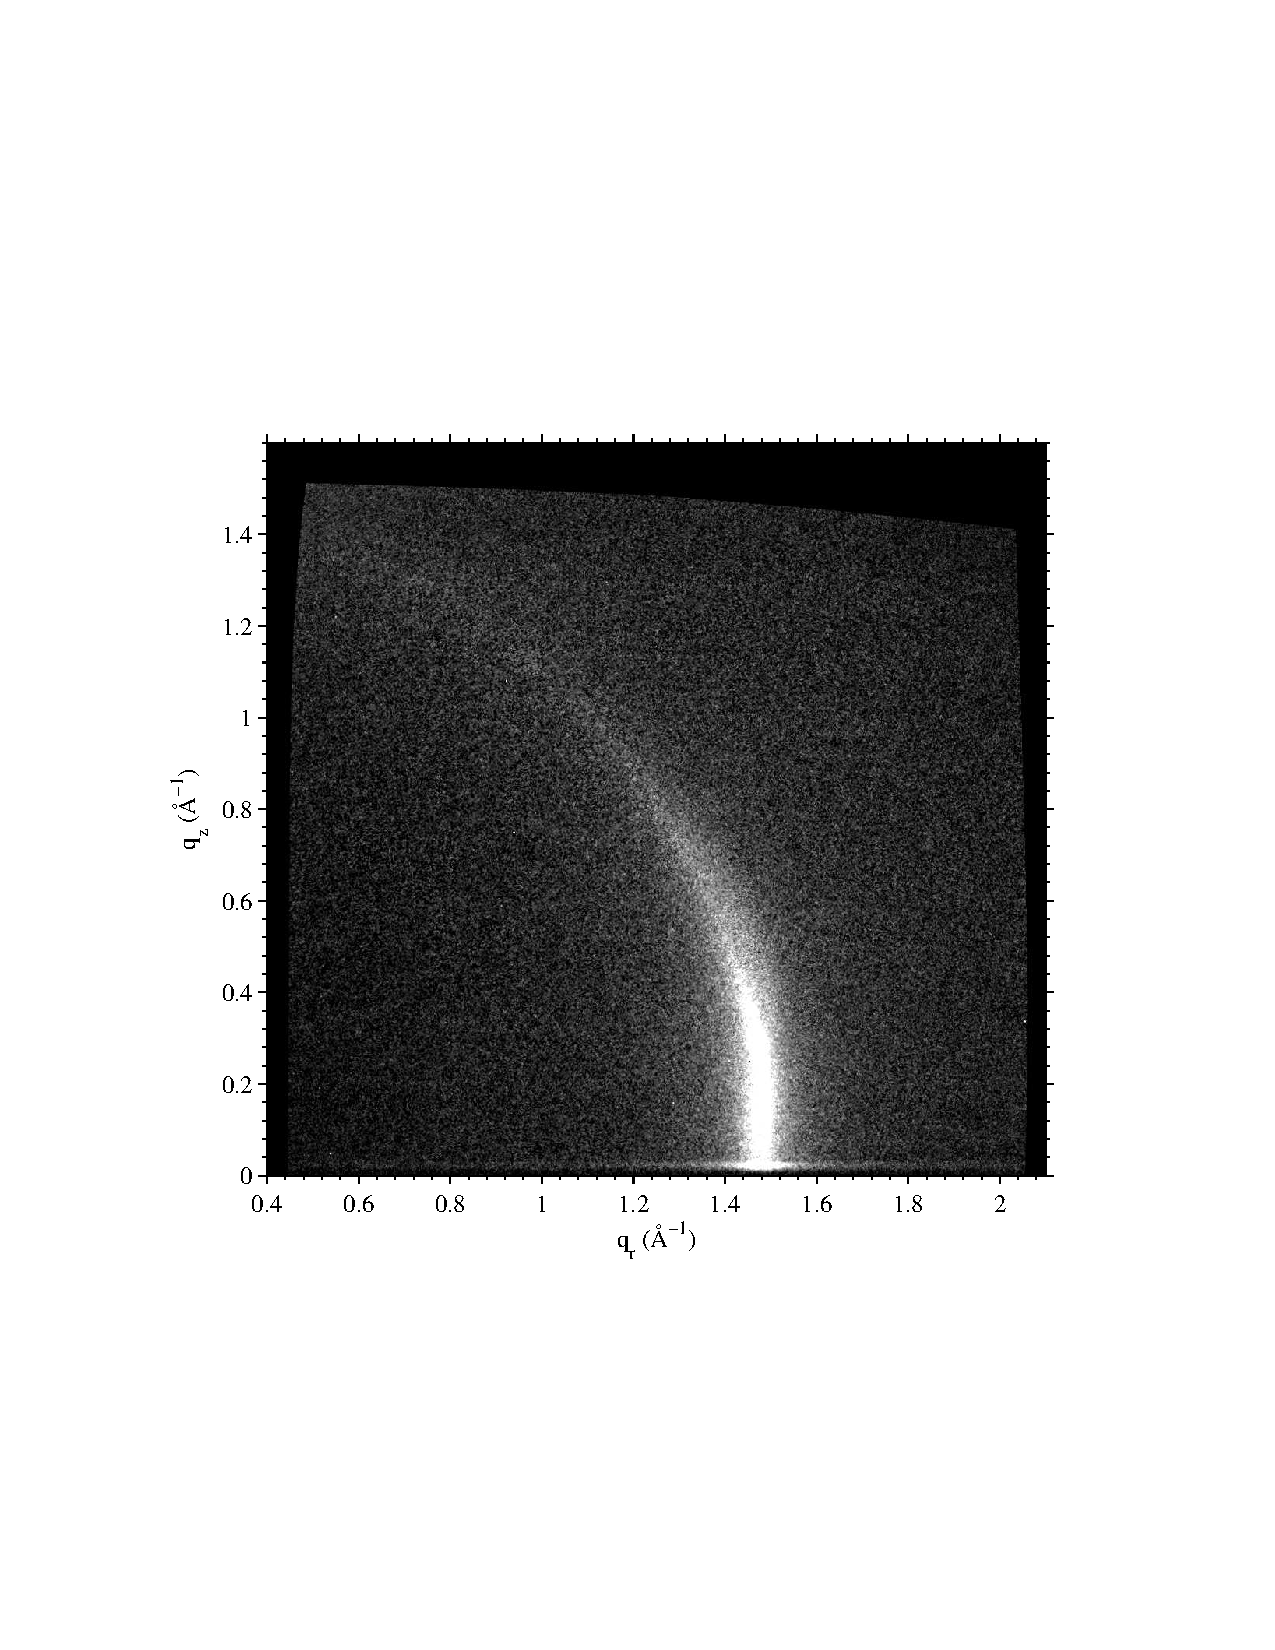
\includegraphics[trim=50 170 50 200,clip,width=0.45\textwidth]{figures/ripple/dmpc1_046}
  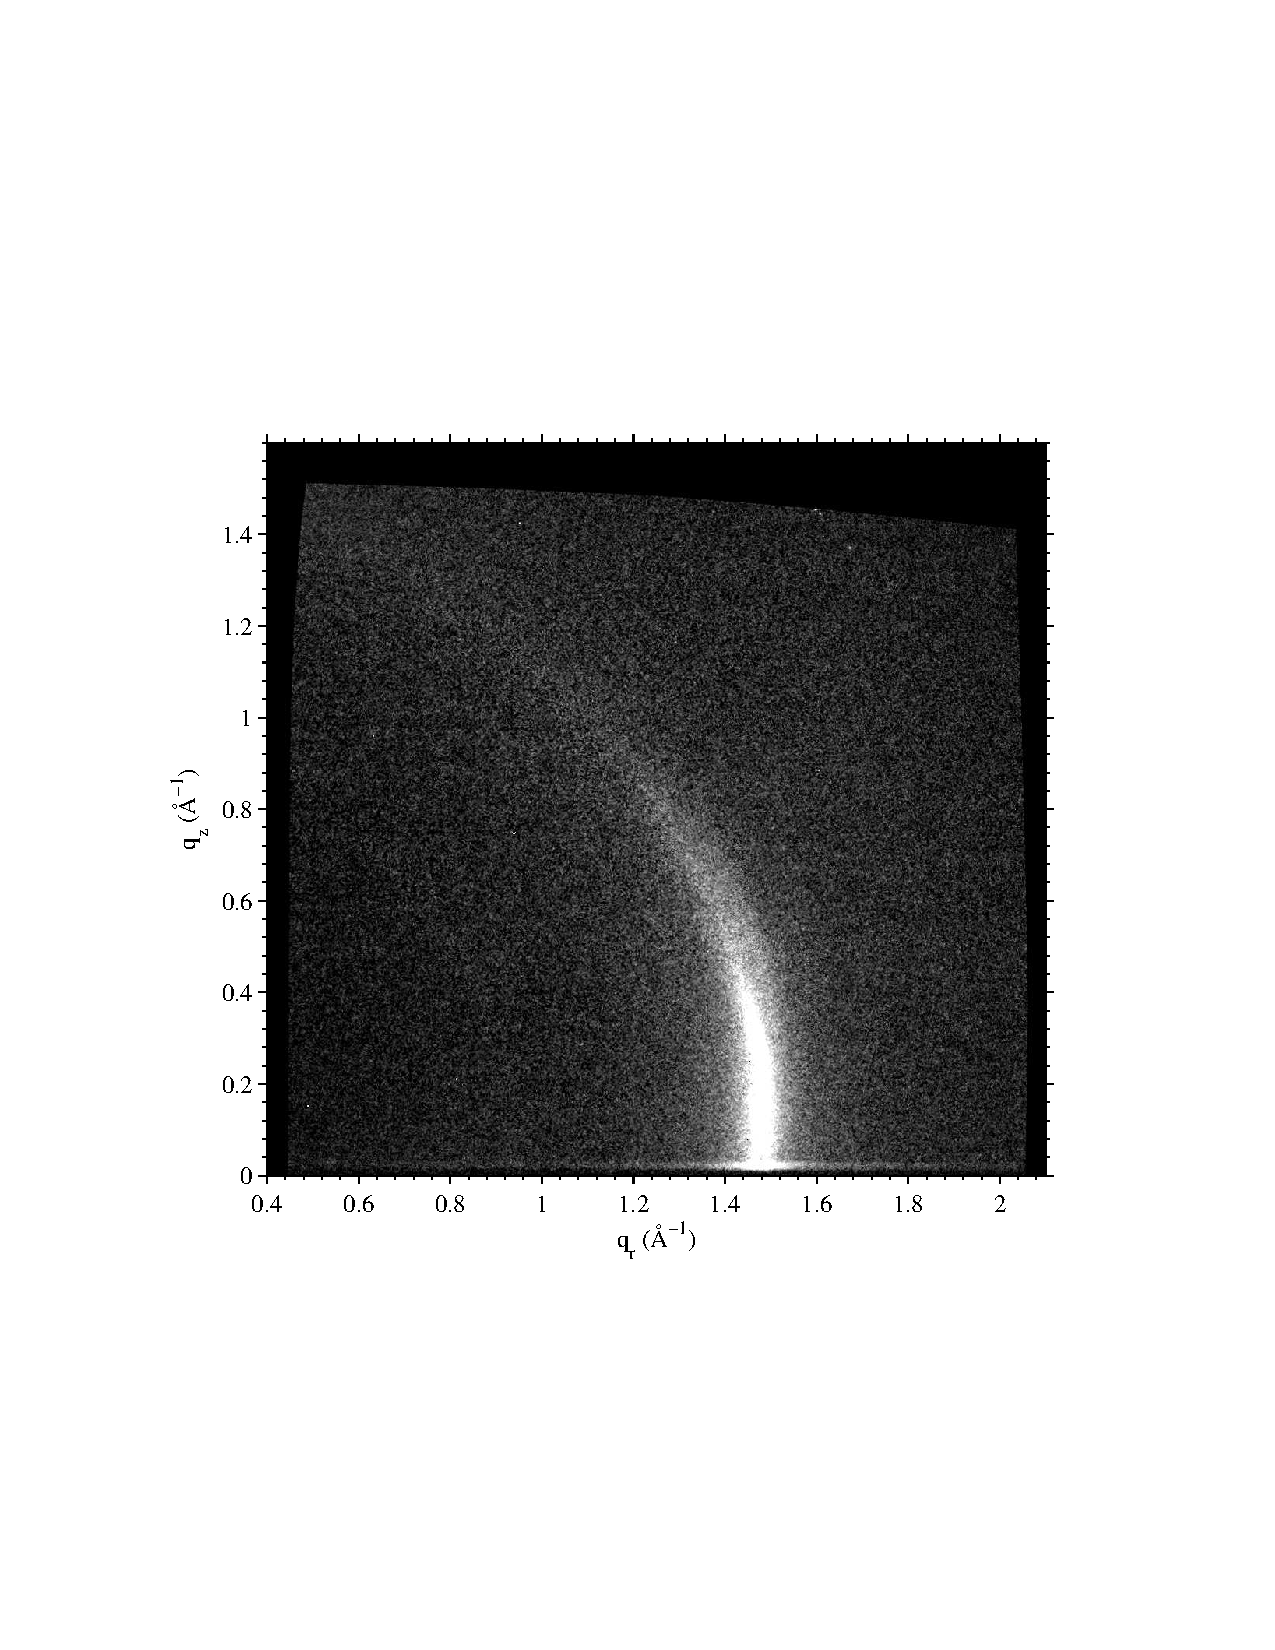
\includegraphics[trim=50 170 50 200,clip,width=0.45\textwidth]{figures/ripple/dmpc1_052-060}
  \caption{NGIWAXS of the DMPC ripple phase for $D$ = 59.2 \AA\ (left)
  and 60.8 \AA\ (right). The angle of incidence $\omega$ was 0.2\textdegree.
  The black regions around the edge of each image are the $q$-space that 
  was not probed. The distorted, non rectangular shape of the probed $q$-space
  signifies non-linear relation between the CCD space and sample $q$-space.}
  \label{fig:NGIWAXS}
\end{figure}

\begin{figure}
  \centering
  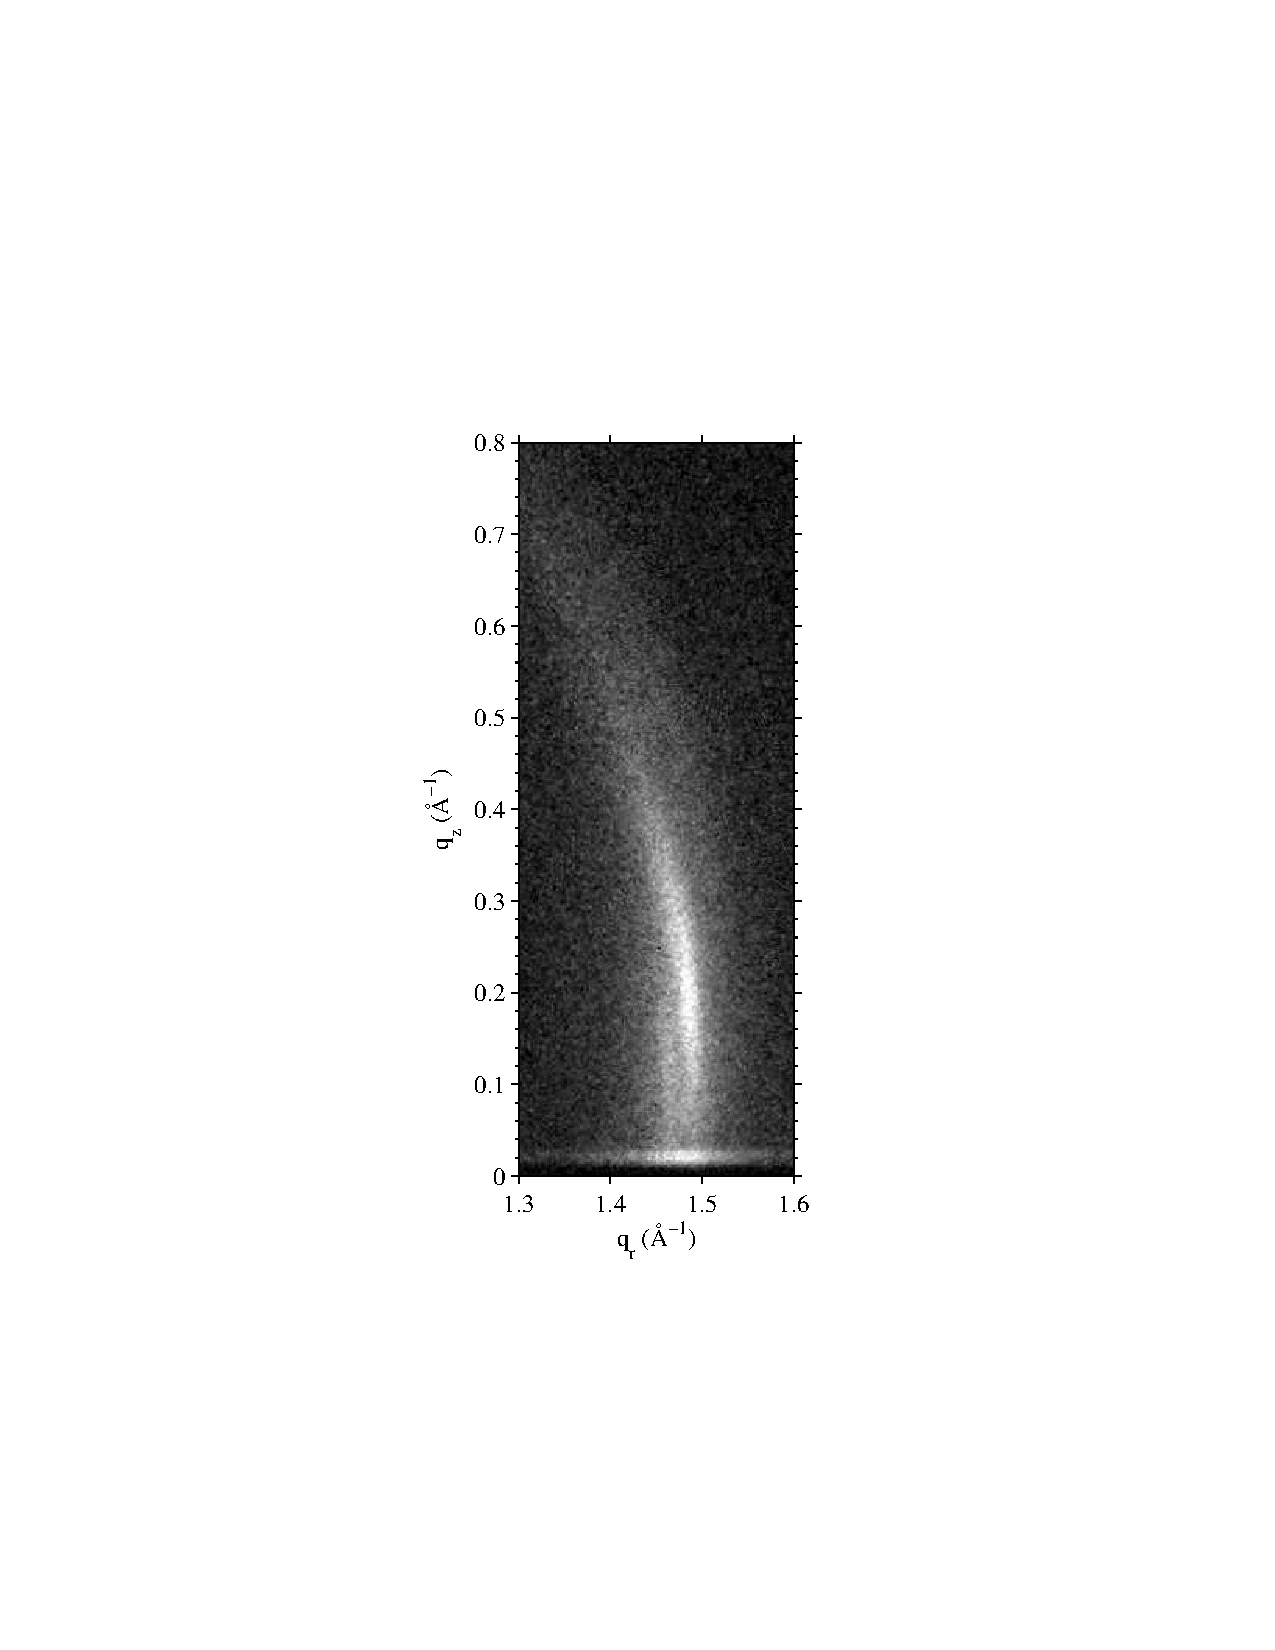
\includegraphics[trim=100 170 100 170,clip,width=\textwidth]{figures/ripple/dmpc1_enlarge}
  \caption{Enlarged view of the right image in Fig.~\ref{fig:NGIWAXS}. To show 
  smaller features around the peak, a different contrast is used.}
  \label{fig:NGIWAXS_enlarge}
\end{figure}

\begin{figure}
  \centering
  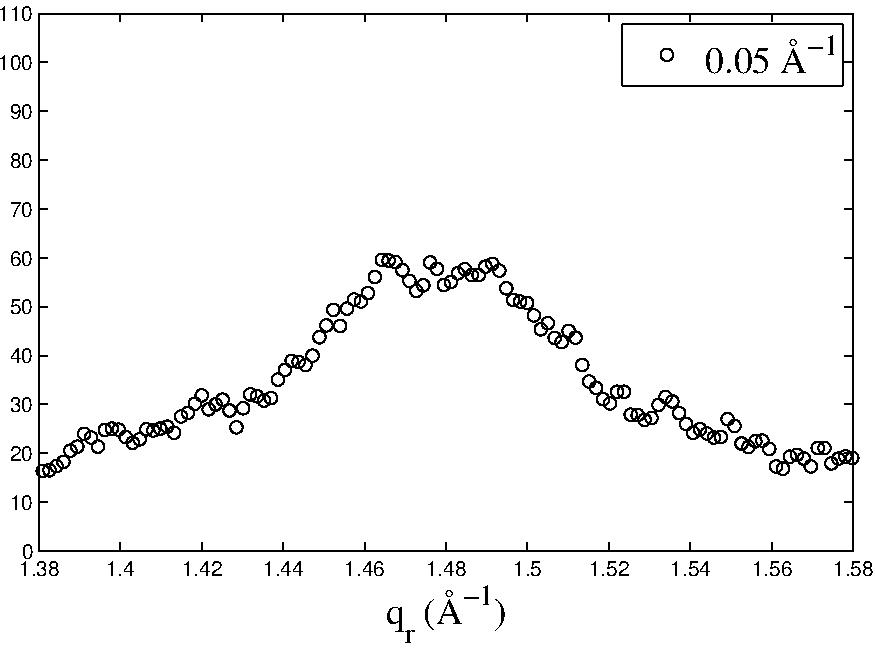
\includegraphics[width=0.3\textwidth]{figures/ripple/qrplot0}
  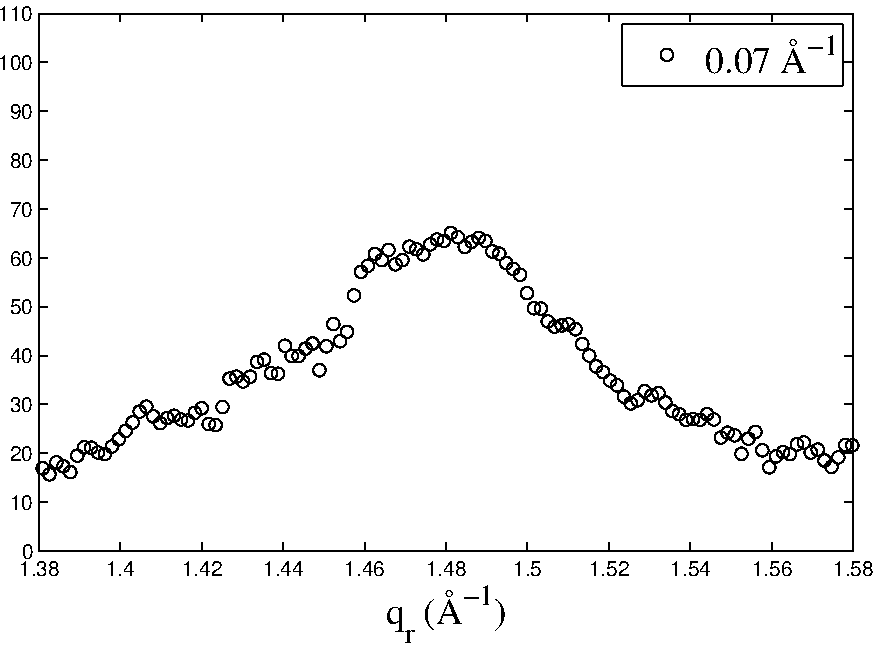
\includegraphics[width=0.3\textwidth]{figures/ripple/qrplot1}
  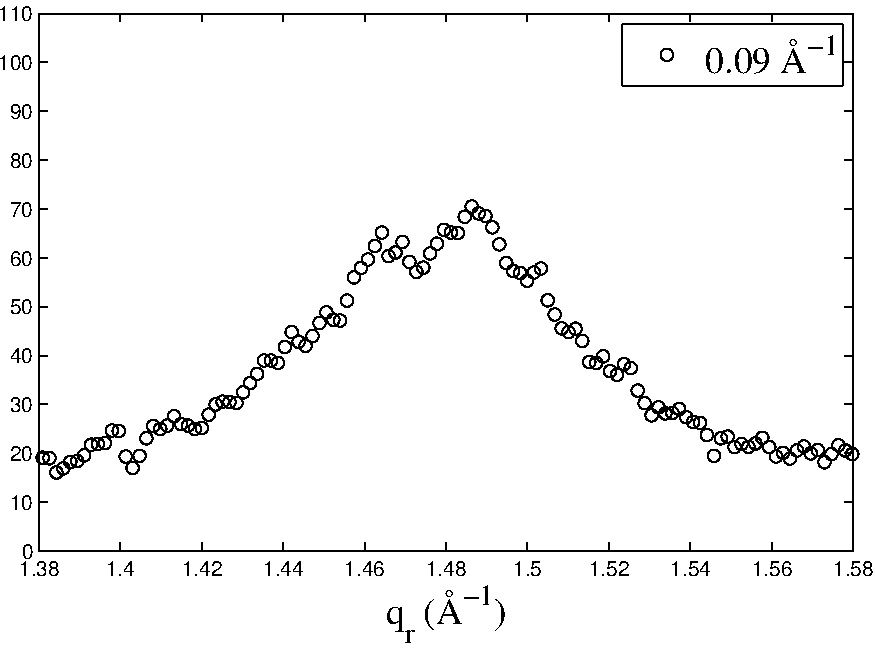
\includegraphics[width=0.3\textwidth]{figures/ripple/qrplot2}
  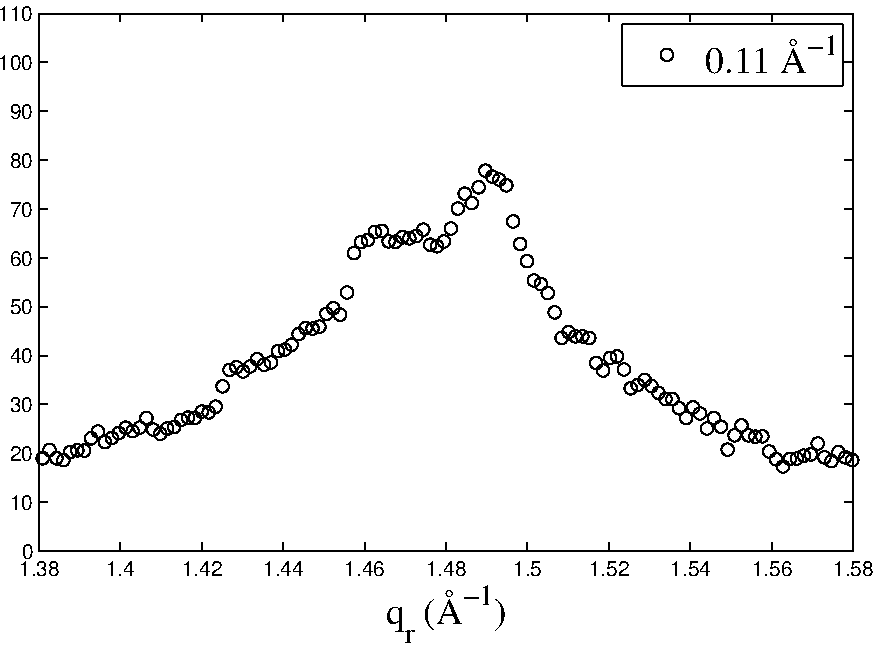
\includegraphics[width=0.3\textwidth]{figures/ripple/qrplot3}
  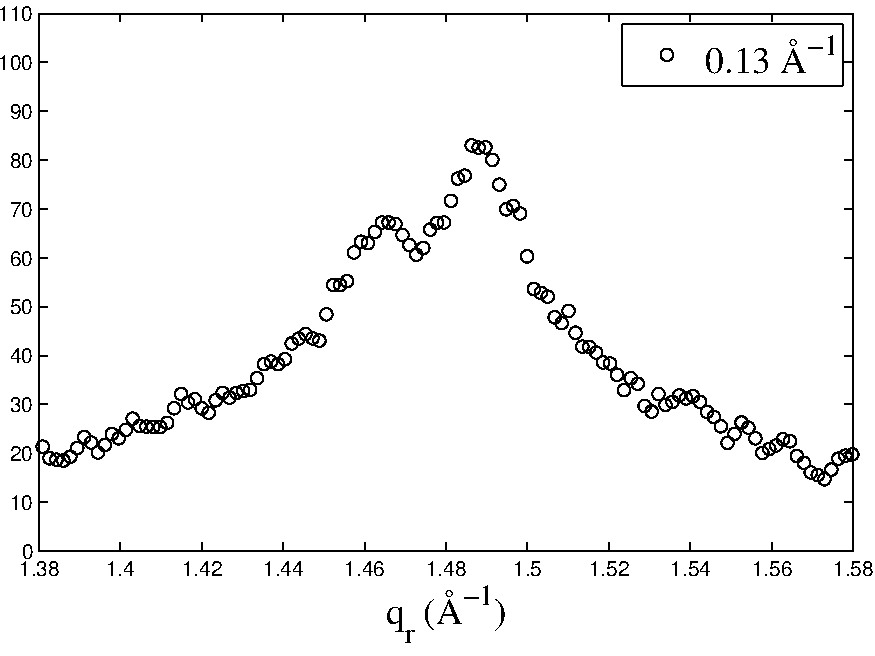
\includegraphics[width=0.3\textwidth]{figures/ripple/qrplot4}
  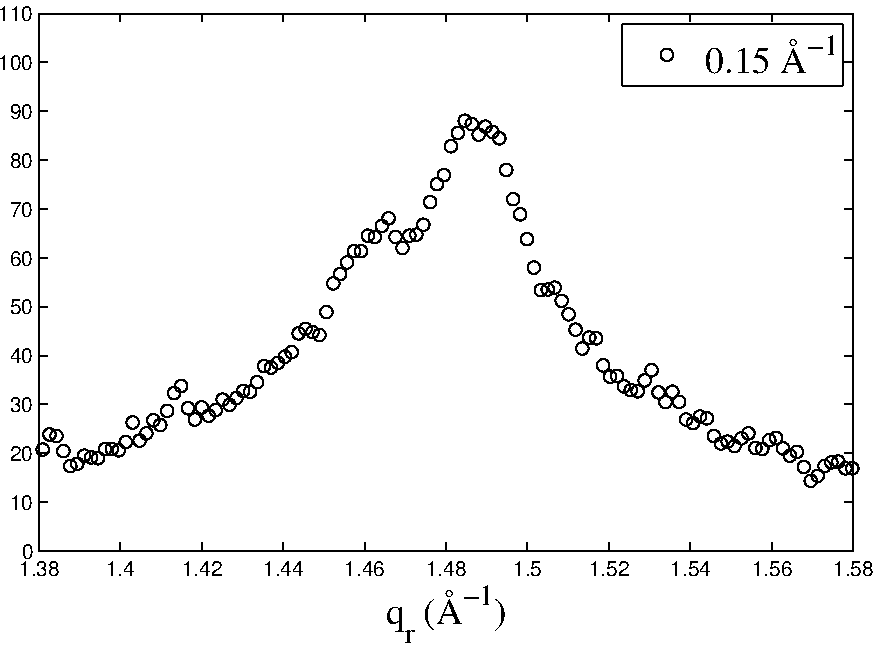
\includegraphics[width=0.3\textwidth]{figures/ripple/qrplot5}
  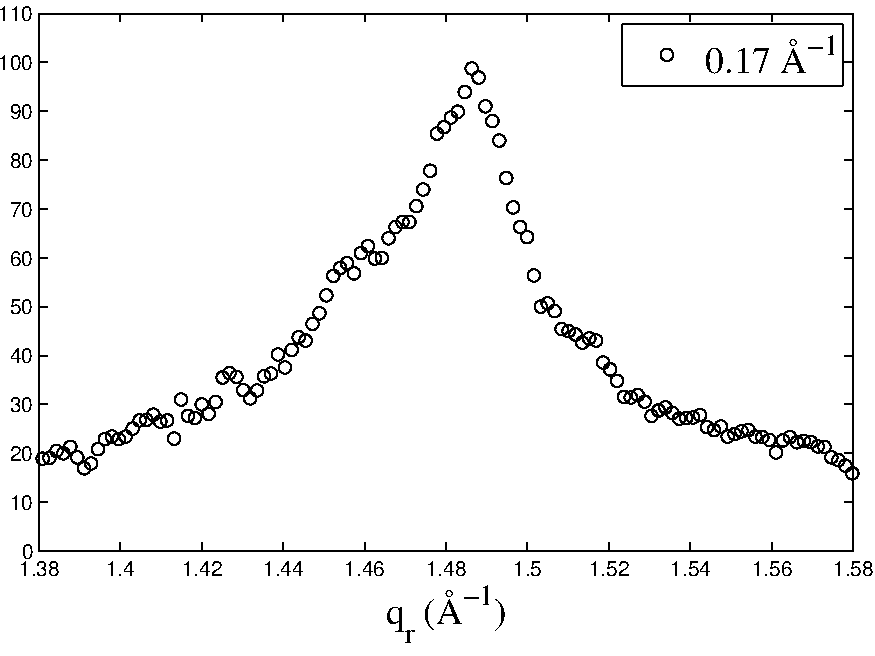
\includegraphics[width=0.3\textwidth]{figures/ripple/qrplot6}
  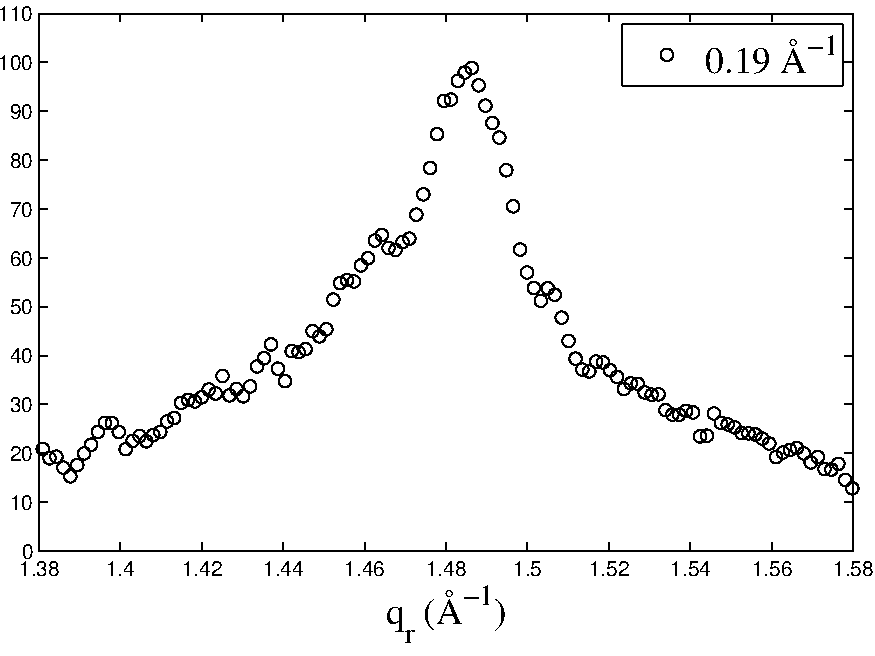
\includegraphics[width=0.3\textwidth]{figures/ripple/qrplot7}
  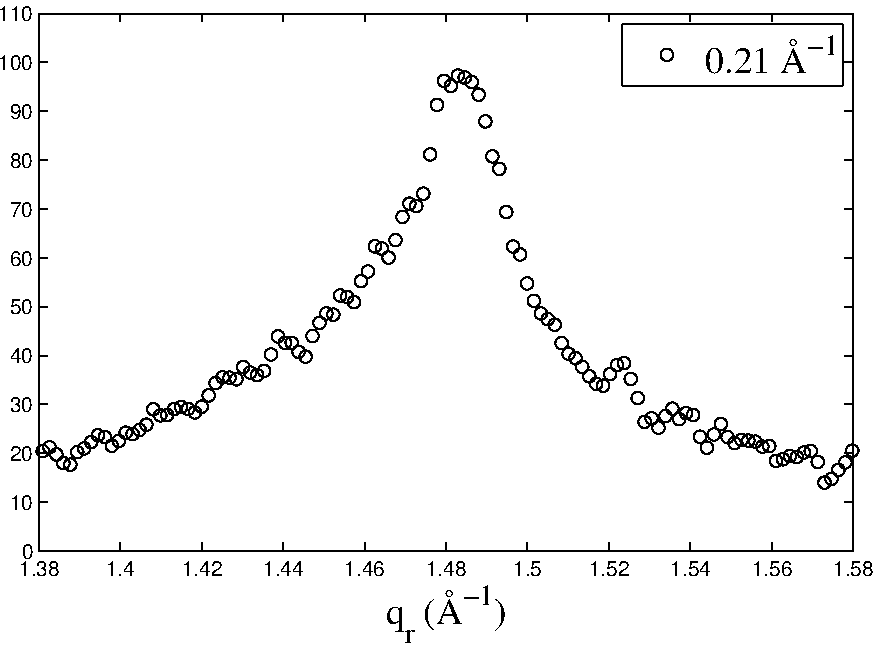
\includegraphics[width=0.3\textwidth]{figures/ripple/qrplot8}
  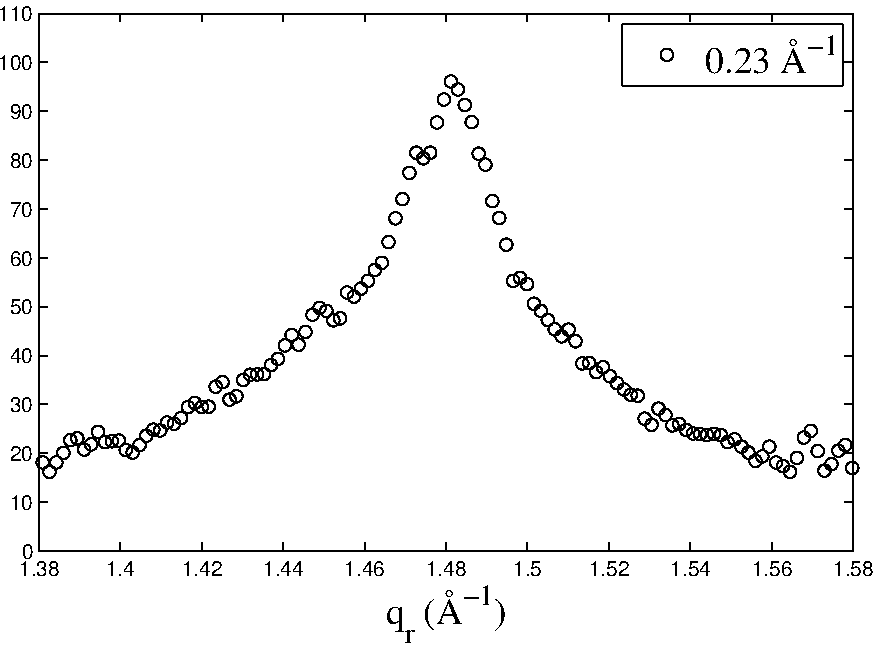
\includegraphics[width=0.3\textwidth]{figures/ripple/qrplot9}
  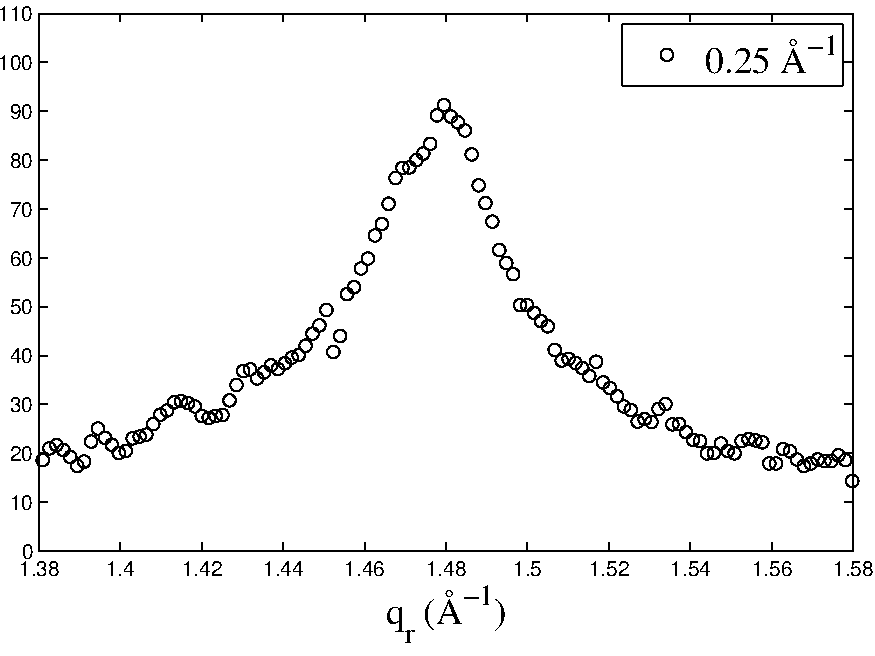
\includegraphics[width=0.3\textwidth]{figures/ripple/qrplot10}
  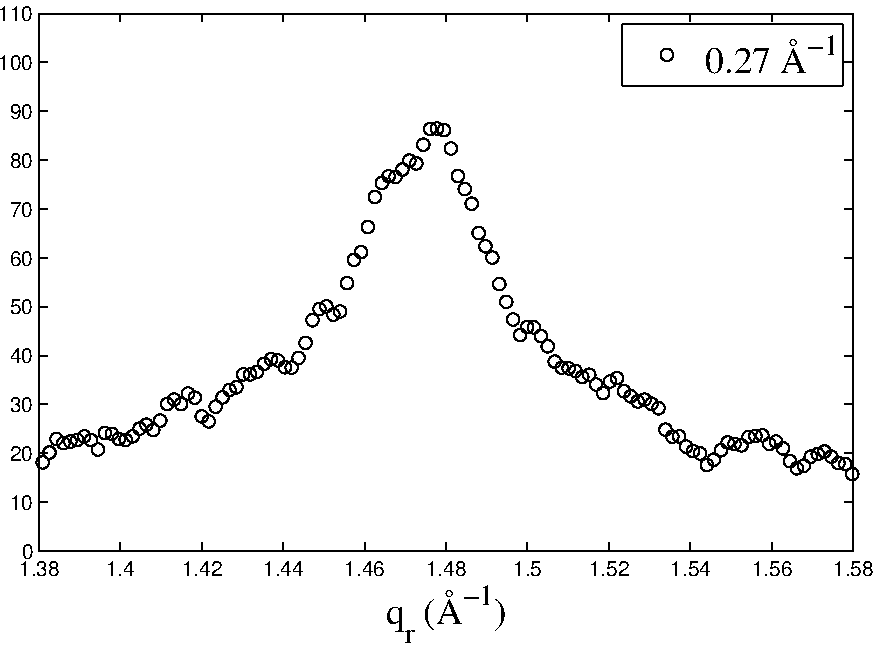
\includegraphics[width=0.3\textwidth]{figures/ripple/qrplot11}
  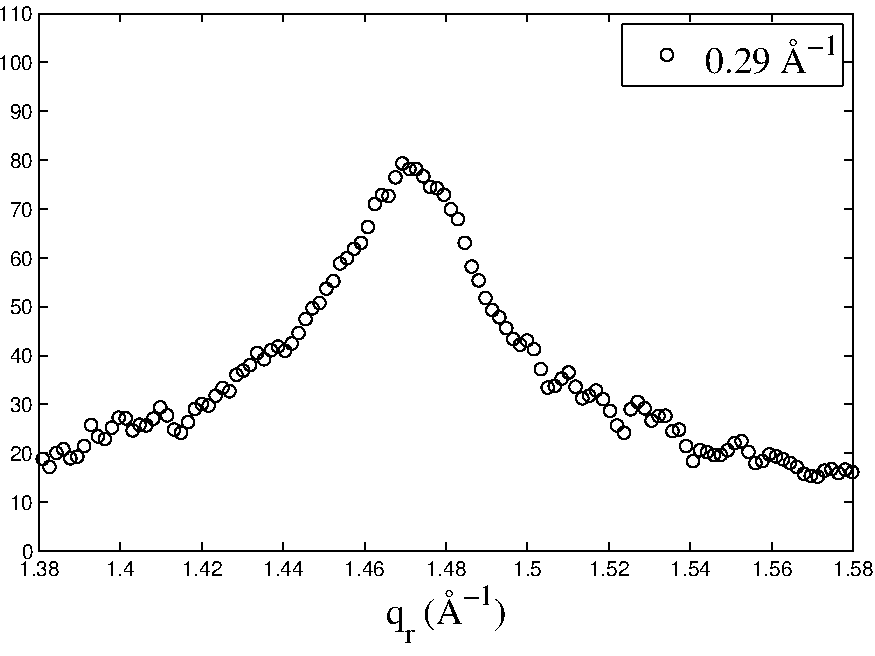
\includegraphics[width=0.3\textwidth]{figures/ripple/qrplot12}
  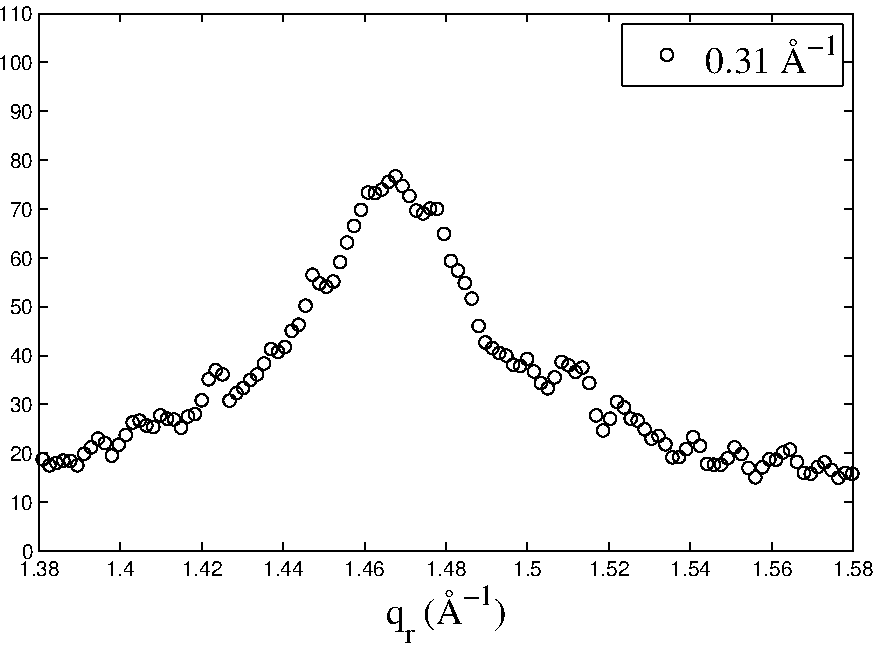
\includegraphics[width=0.3\textwidth]{figures/ripple/qrplot13}
  \caption{$q_r$ swaths, each averaged over 0.02 \AA$^{-1}$. 
  The center $q_z$ value of a swatch is shown in the figure legends.}
  \label{fig:qrplots}
\end{figure}

(some thought) Can we say that
the observed arc like scattering is not the mosaic spread, but
true sample scattering? Comment on the widths of the peaks observed.
Possibly make use of both low and high resolution data.
Apply the absorption correction. Show q swaths for various $\phi$.

\subsection{Transmission WAXS}
Convert the image to $q$-space.
No strong order on the equator. 
Compare to NGIWAXS and comment on the absorption effect
in NGIWAXS data.

\section{Discussion}
Comparison with previous unoriented/oriented stuff.

\section{Conclusion}
Future possible experiments
include the high resolution transmission experiment, where both geometric 
broadening and energy dispersion are minimized. The expected resolution 
is the width of the X-ray beam, which is about 3 pixels. This experiment 
doubles the best resolution achieved in this work. 
Another slightly different high resolution experiment is to use silicon 
crystal analyzer downstread of the sample, which completely remove geoemtric
boradening. The downside of this type of high resolution experiment is that
only one point in q-space is probed at any given exposure, so to get a full
2D map of wide angle scattering is time consuming.  
